


\documentclass{article}

\usepackage{amsmath, bm}
\usepackage{graphicx}
\usepackage{amssymb}
\usepackage{float}
\usepackage{caption}
\usepackage{subcaption}
\usepackage{hyperref}
\usepackage{tikz}
\usepackage{pgfplots}
\usepackage{enumitem}
\usepackage{hyperref}
\usepackage{tikz}
\usepackage{pgfplots}
\usepackage{listings}
\usepackage{xcolor}
\usepackage[margin=1in]{geometry}
\usepackage{savetrees}

% Custom subsection numbering
\renewcommand{\thesubsection}{\roman{subsection})}
\renewcommand{\thesubsubsection}{\alph{subsubsection})}

% Set depth for numbering and TOC
\setcounter{secnumdepth}{3}
\setcounter{tocdepth}{3}

% Explicit formatting with indentation
\usepackage{titlesec}

% Indent subsection titles (Roman numerals)
\titleformat{\subsection}
  {\normalfont\normalsize\bfseries}
  {\hspace{1.5em}\thesubsection}{1em}{}

% Indent subsubsection further (nested under subsection)
\titleformat{\subsubsection}
  {\normalfont\normalsize\itshape}
  {\hspace{2em}\thesubsubsection}{1em}{}

\usetikzlibrary{calc}
\usetikzlibrary{angles,quotes} % for pic
\usetikzlibrary{patterns,snakes}
\usetikzlibrary{arrows}
\usetikzlibrary{shapes.geometric, arrows}
\tikzset{>=latex} % for LaTeX arrow head

\setlength{\parskip}{\baselineskip}%
\setlength{\parindent}{0pt}%
\linespread{0.9}


\lstset{
  language=Matlab,
  basicstyle=\ttfamily\small,
  keywordstyle=\color{blue}\bfseries,
  commentstyle=\color{green!60!black},
  stringstyle=\color{orange},
  numbers=left,
  numberstyle=\tiny\color{gray},
  stepnumber=1,
  numbersep=10pt,
  breaklines=true,
  backgroundcolor=\color{gray!10},
  captionpos=b
}
\tikzset{
    cg/.style={
        draw,
        circle,
        thick,
        minimum size=0.2cm, % Adjust the size of the circle
        inner sep=0,      % Remove extra padding
        append after command={
            \pgfextra{
                \draw[thick] (\tikzlastnode.south) -- (\tikzlastnode.north);
                \draw[thick] (\tikzlastnode.west) -- (\tikzlastnode.east);
            }
        }
    }
}

\tikzstyle{startstop} = [rectangle, rounded corners, minimum width=3cm, minimum height=1cm,text centered, draw=black, fill=red!30]
\tikzstyle{process} = [rectangle, minimum width=3cm, minimum height=1cm, text centered, draw=black, fill=orange!30]
\tikzstyle{decision} = [diamond, minimum width=3cm, minimum height=1cm, text centered, draw=black, fill=green!30]
\tikzstyle{io} = [trapezium, trapezium left angle=70, trapezium right angle=110, minimum width=3cm, minimum height=1cm, text centered, draw=black, fill=blue!30]
\tikzstyle{arrow} = [thick,->,>=stealth]

\begin{document}

\title{4F2 Robust and Nonlinear control}
\author{5735G}
\date{Feburary 2025}
\maketitle 

\begin{center}
    \textbf{Summary} \\
    
\end{center}

\section{Stable and oscillatory recurrent neural networks}

\begin{equation}
    \dot{x} = f(x) + B_u u + B_w w = \begin{bmatrix}
        -10z_1 + 10y \\
        -100z_2 + 100y \\
        -y + \varphi(w_1z_1 + w_2z_2 + w_3y)
    \end{bmatrix} + \begin{bmatrix}
        0 \\ 0 \\ 1
    \end{bmatrix} r
\end{equation}

\begin{equation}
    y = \psi(x) + D_u u + D_w w = y
\end{equation}

The nonlinear activation function is defined as $\varphi(x) = \tanh(x)$ jacobians are defined as
\begin{equation}
    \partial f(x) = \begin{bmatrix}
        -10 & 0 & 10 \\
        0 & -100 & 100 \\
        w_1 \varphi'(w^T x) & w_2 \varphi'(w^T x) & -1 + w_3 \varphi'(w^T x)
    \end{bmatrix} \quad \text{ and } \quad \partial \psi(x) = \begin{bmatrix}
        0 & 0 & 1
    \end{bmatrix}
\end{equation}

\subsection{Weights to satisfy a bounded differential gain}

The derivative $\varphi'$ acts like a sigmoid which satisfies the condition
\begin{equation}
    0 \leq \varphi'(x) \leq 1 \quad \forall x \in \mathbb{R}
\end{equation}

This allows us to define a complex hull which contains $\partial f(x)$:

\begin{equation}
    \partial f(x) \in \{ A_0 + sA_1 | s \in [0,1]\}
\end{equation}

This allows us to define two linear matrix inequalities (LMIs) to guarantee differential gain. 

\begin{equation}
    \left[
    \begin{array}{cc}
    A_i^T P + P A_i + 2\lambda P + \frac{1}{\gamma} \partial \varphi(x)^T \varphi(x) & PB \\
    B^T P & -\gamma I
    \end{array}
    \right] \leq 0.
\end{equation}

Values of $ w = \begin{bmatrix} 0.1 & 0.1 & 0.1 \end{bmatrix}^T $ were found to give a solution for P and hence satisfy the bounded differential gain condition.
Unit step and harmonic reference signals were applied and the responses can be seen plotted below in figures \ref{fig:11_step} and \ref{fig:11_harmonic}.

\begin{figure}[H]
    \centering
    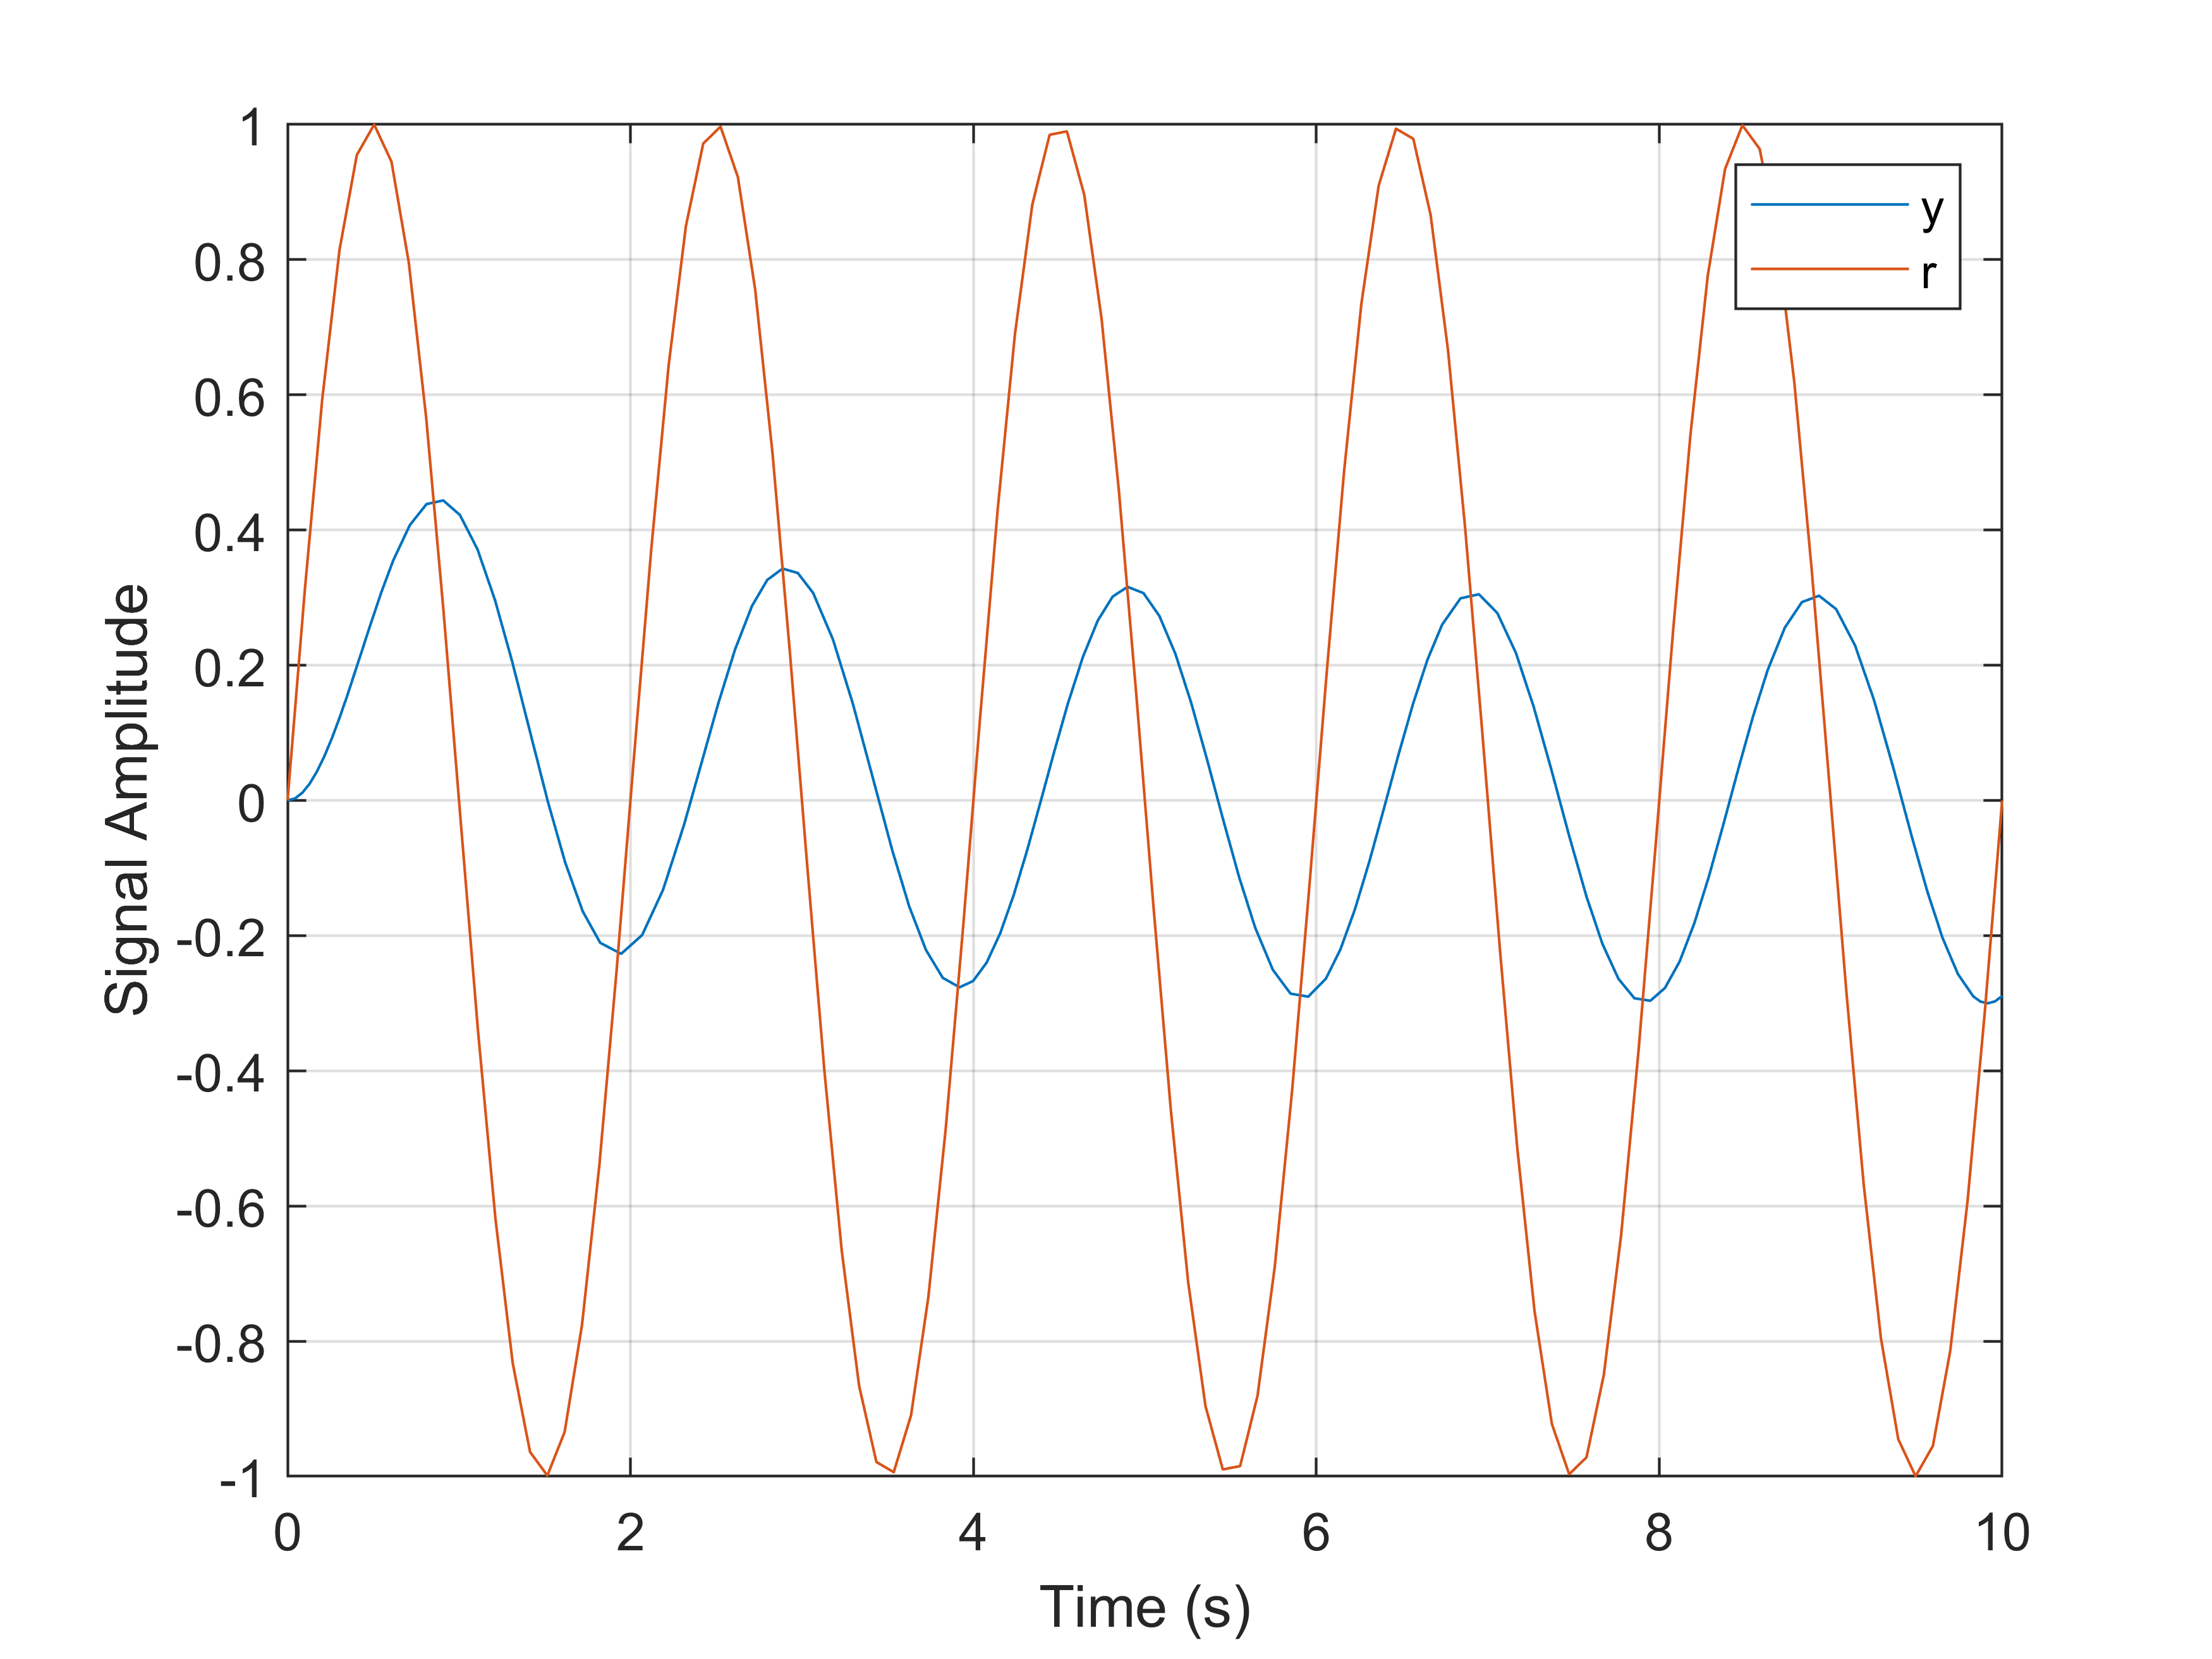
\includegraphics[width=0.5\textwidth]{figures/11_harmonic_reference.png}
    \caption{Response of system to unit step reference signals}
    \label{fig:11_step}
\end{figure}

\begin{figure}[H]
    \centering
    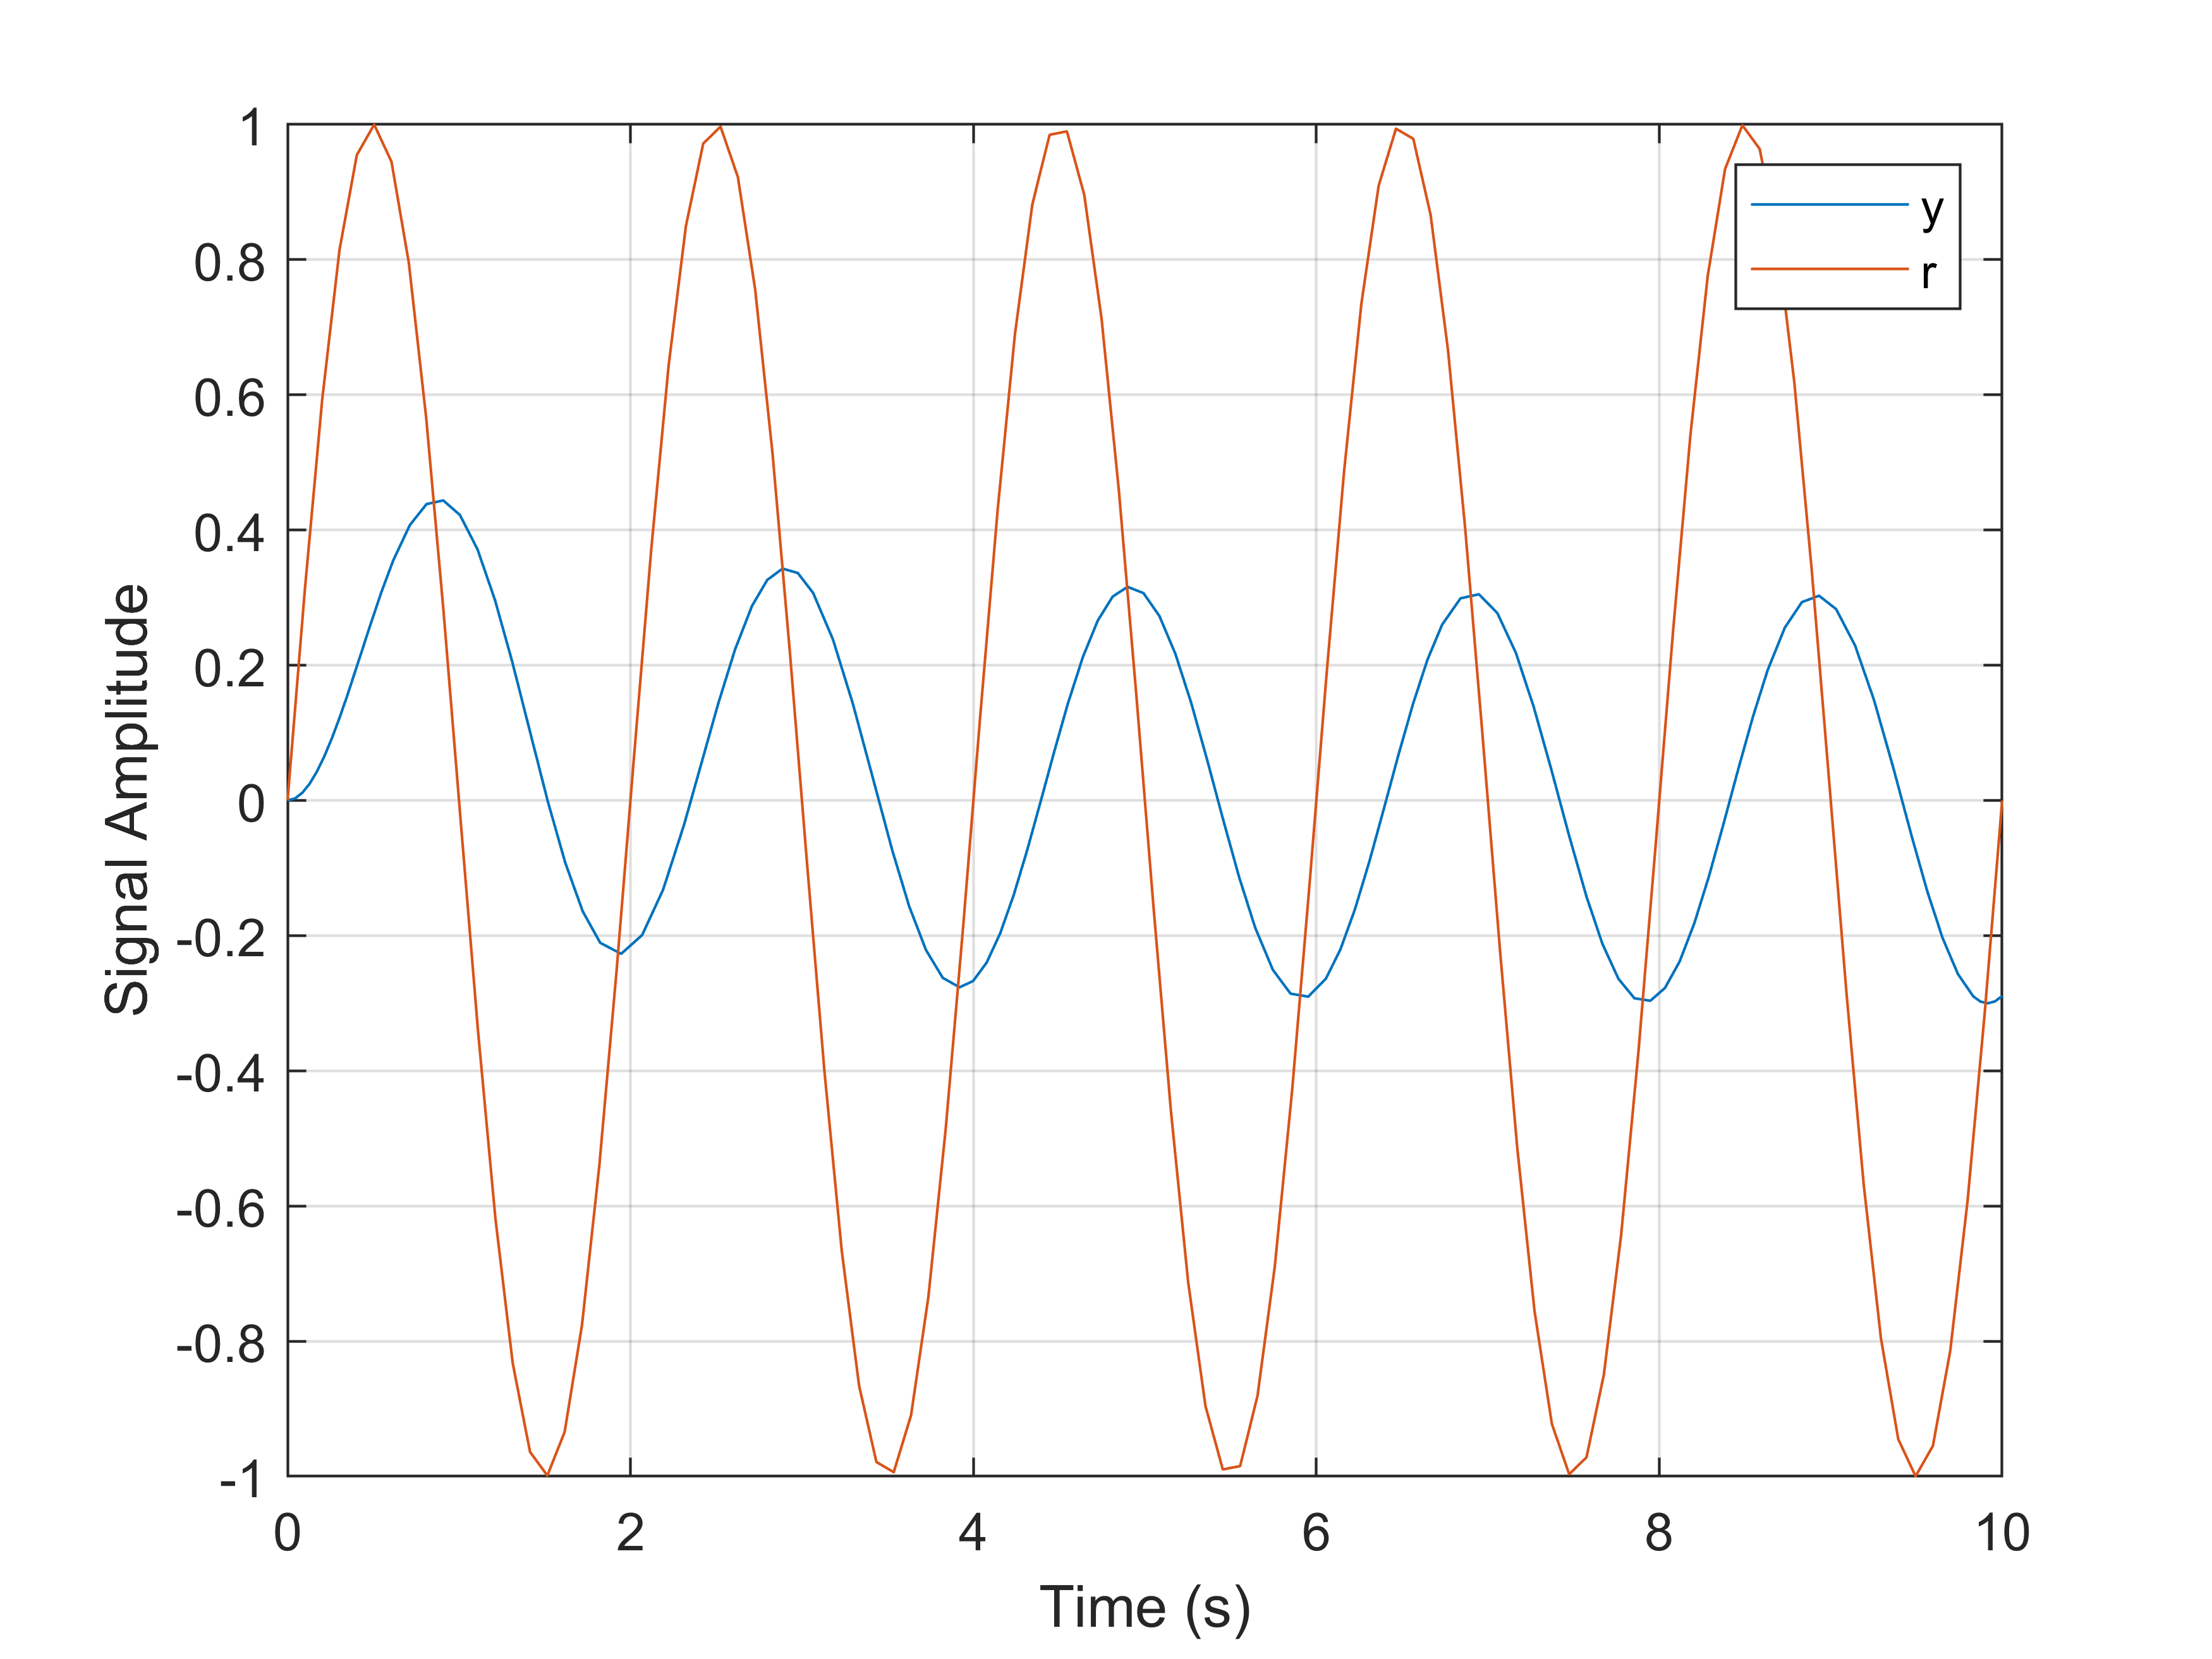
\includegraphics[width=0.5\textwidth]{figures/11_harmonic_reference.png}
    \caption{Harmonic reference signal and systems response}
    \label{fig:11_harmonic}
\end{figure}

The dissipativity LMI in matrix form is given by
\begin{equation}    
\left[
\begin{array}{cc}
\partial f(x)^T P + P \partial f(x) + 2\lambda P & PB - \partial \varphi(x)^T \\
B^T P - \partial \varphi(x) & 0
\end{array}
\right] \leq 0.
\end{equation}

\subsection{Weights for autonomous nonlinear oscillator}
Neglecting the fast dynamics $w_2 = 0$, setting $w_3 = 25$ and taking $r = 0$ allows the
use of phase portrait on the reduced system to understand the variation with $w_1$.
\begin{equation}
    \dot{y} = -y + \varphi(w_1z_1 + 25y) \quad 0.1 \dot{z_1} = -z_1 + y
\end{equation}

\begin{figure}[H]
    \centering
    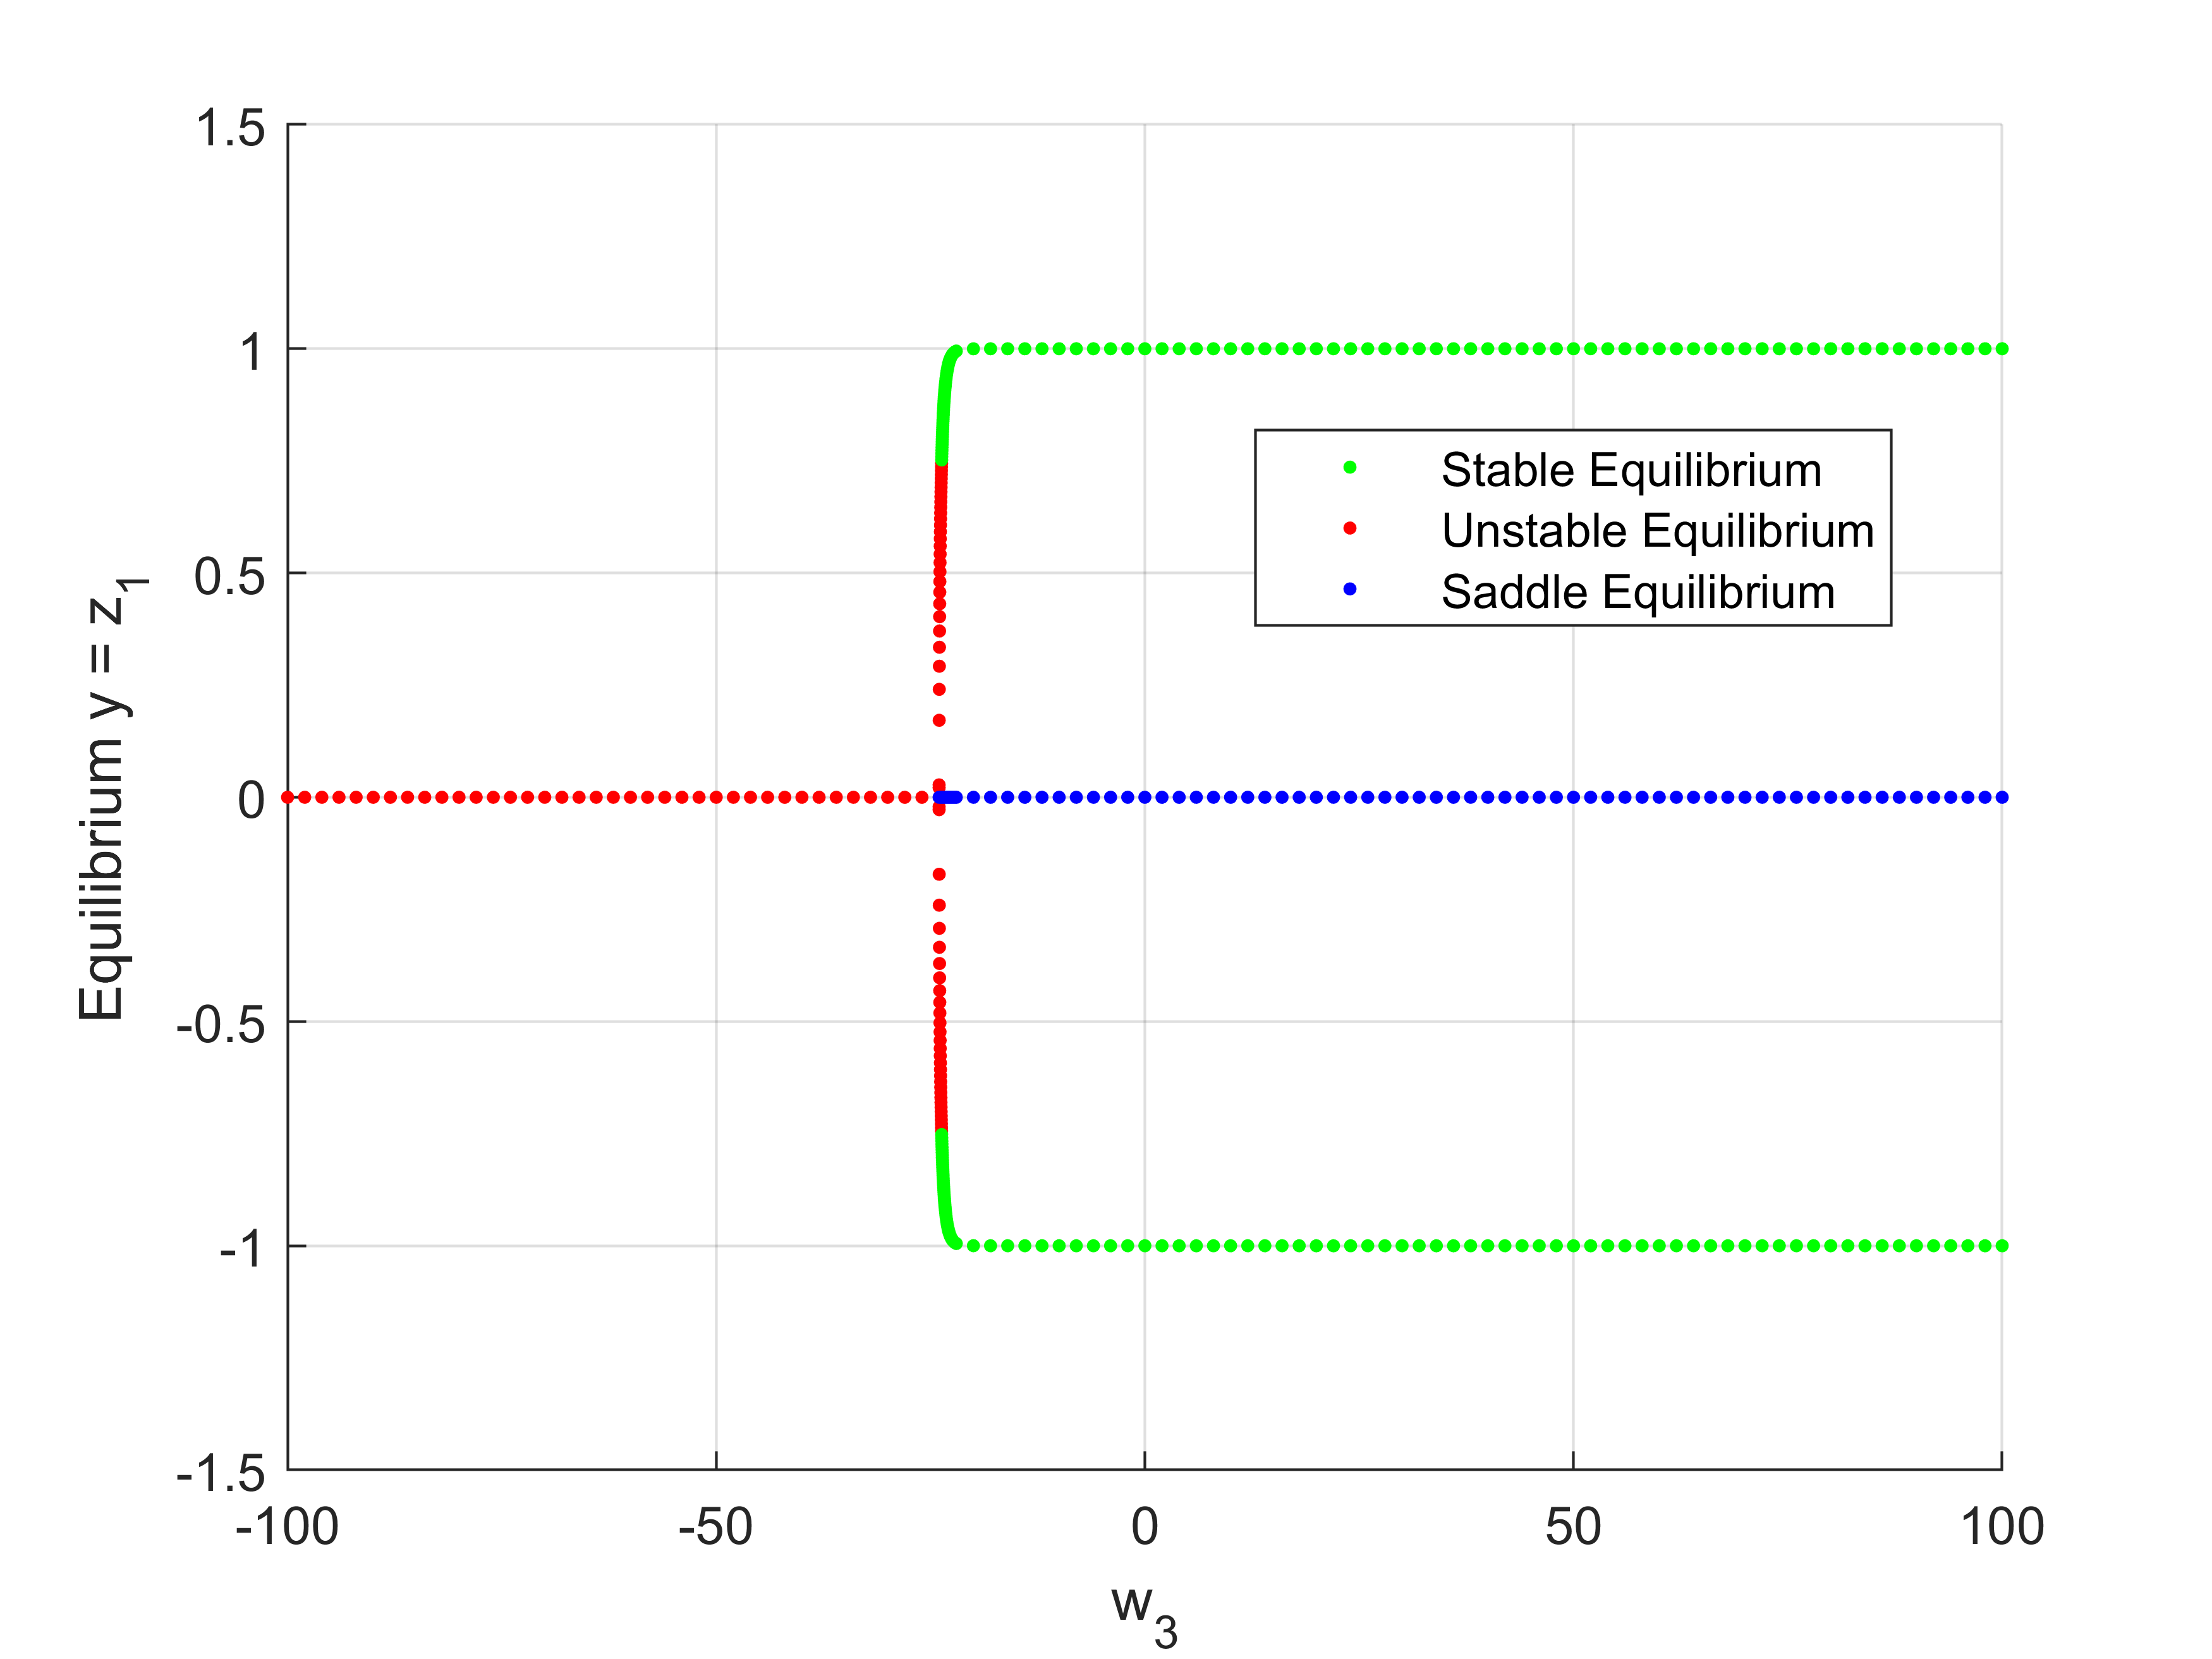
\includegraphics[width=0.5\textwidth]{figures/equilibria_bifurcation.png}
    \caption{Bifurcation of equilibria with varying $w_1$}
    \label{fig:equilibria}
\end{figure}

\begin{figure}[H]
    \centering
    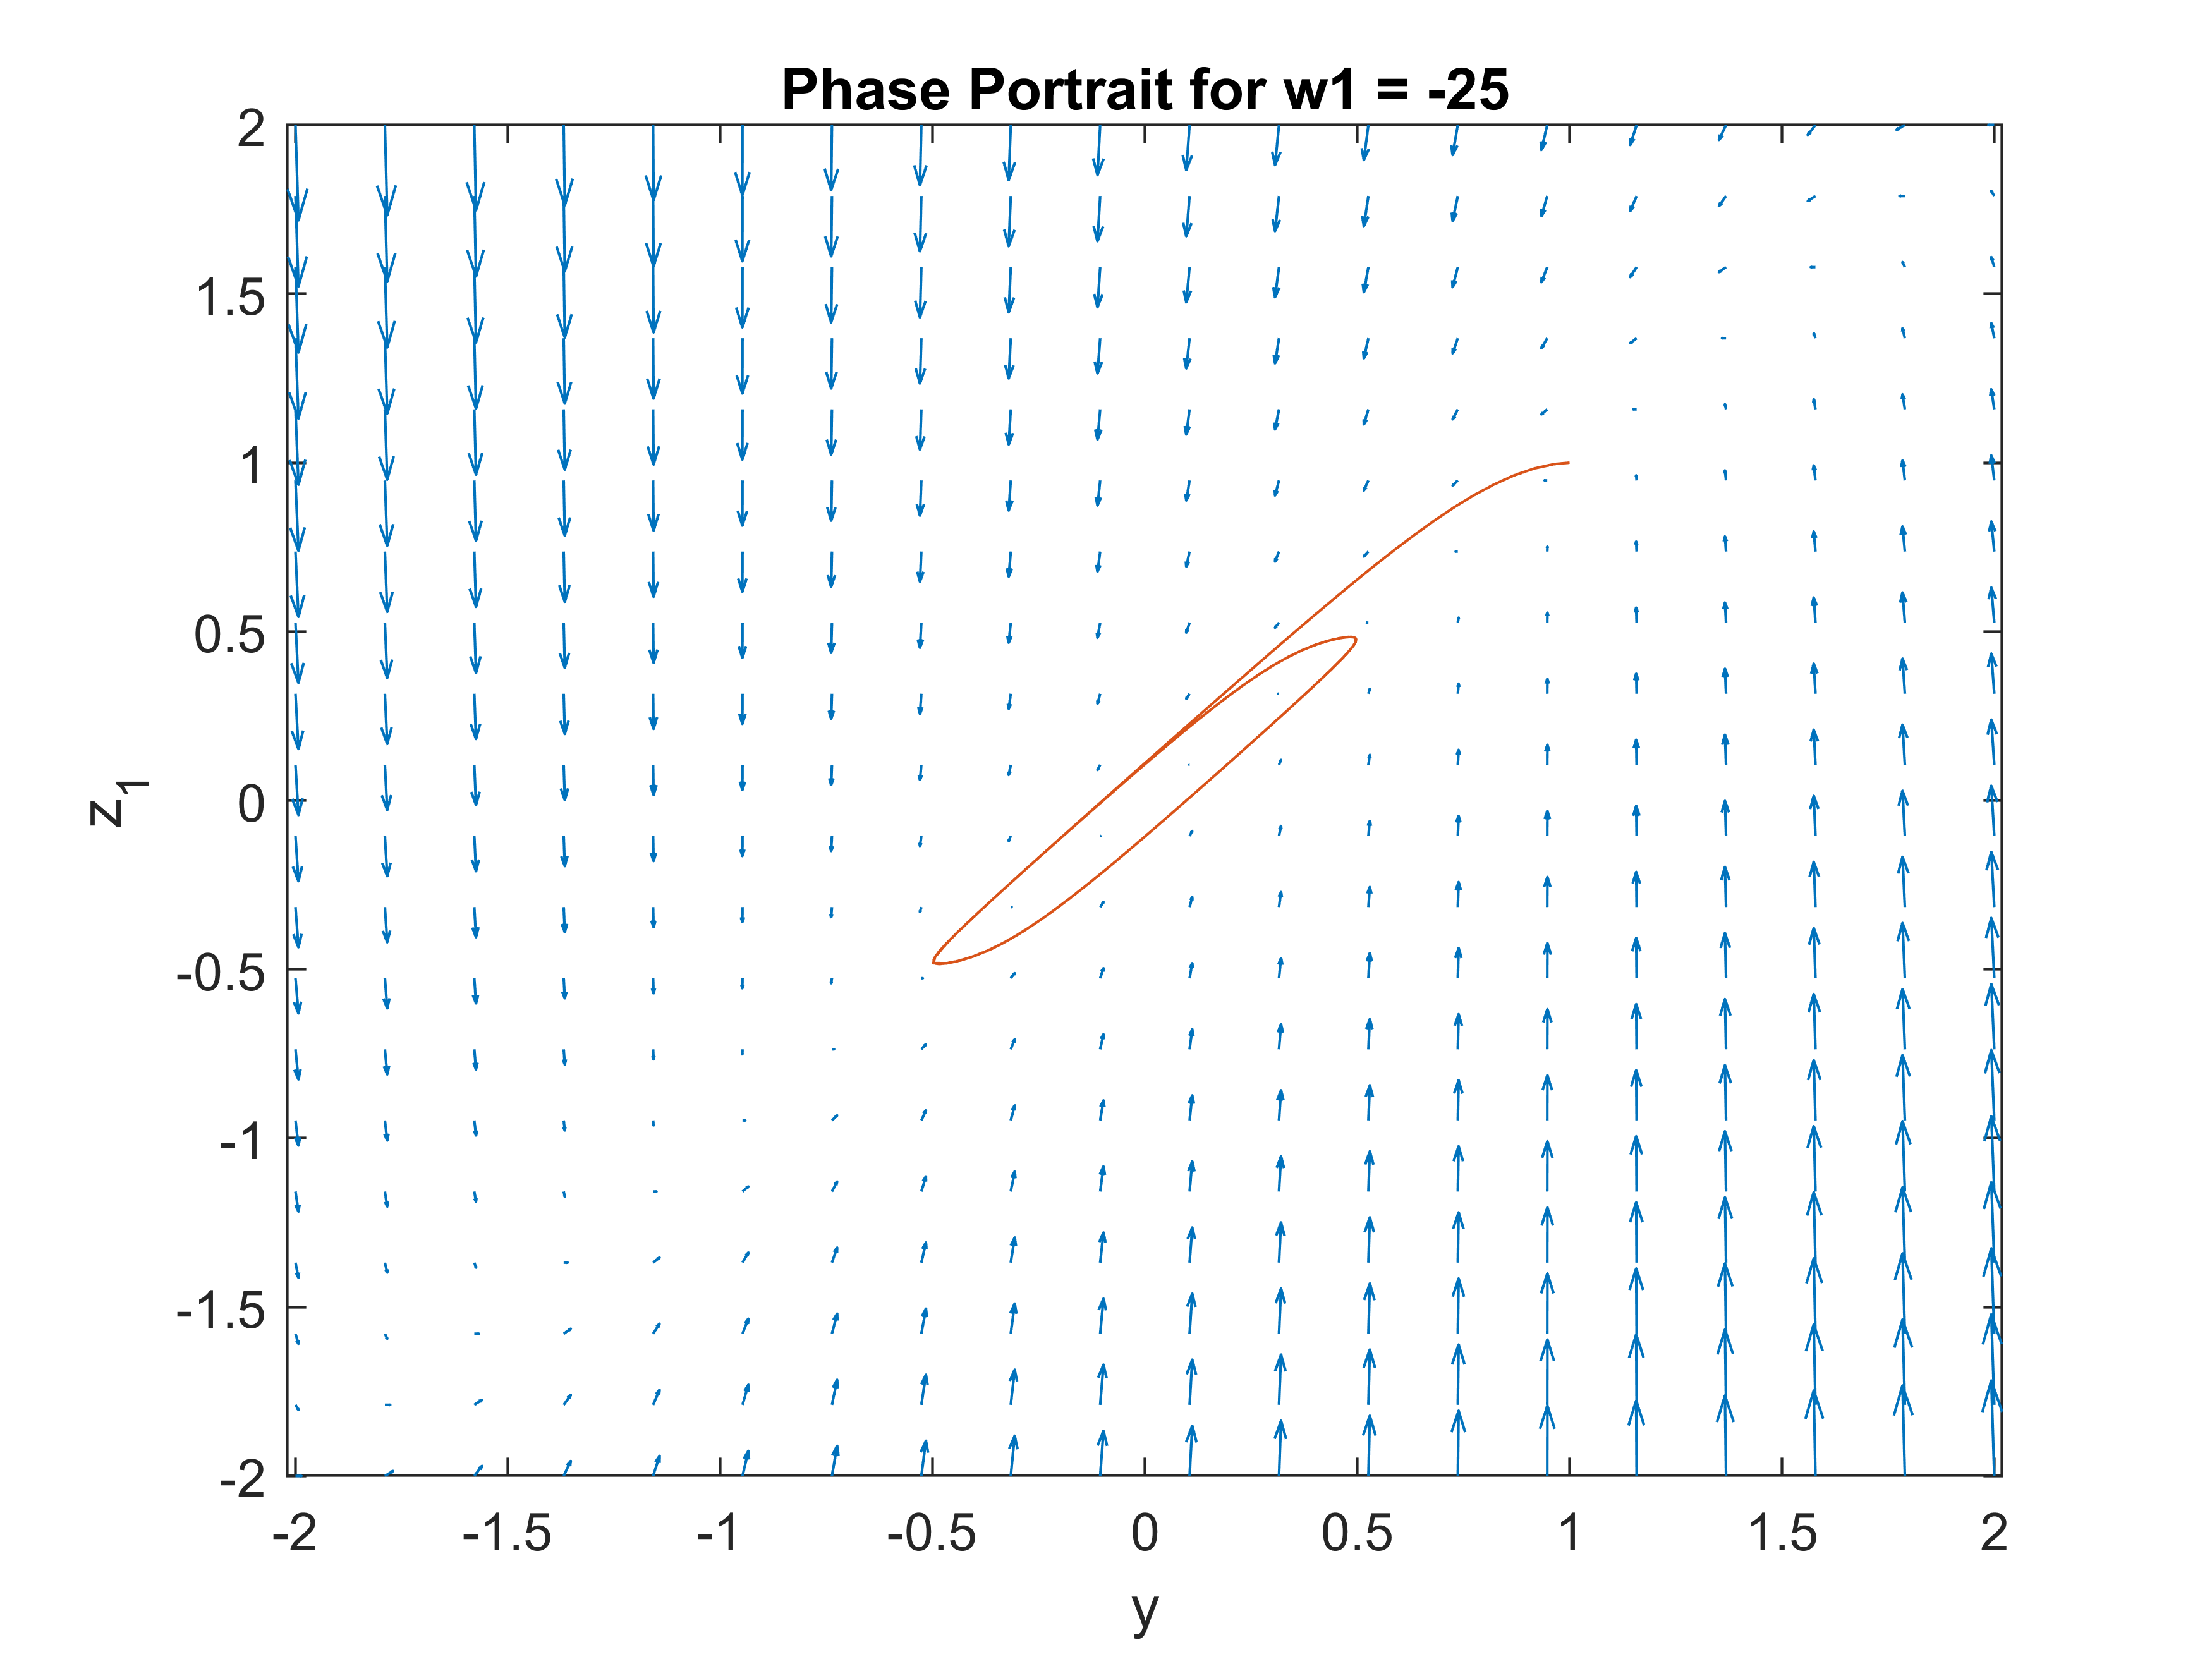
\includegraphics[width=0.5\textwidth]{figures/oscillator_phase_portrait.png}
    \caption{Phase portrait of the autonomous nonlinear oscillator for $w_1 = 100$}
    \label{fig:phase_portrait_w100}
\end{figure}

Feedback LMI:
\begin{equation}
    Y > 0, \quad
    \left[
    \begin{array}{ccc}
    Y \partial f(x)^T + \partial f(x) Y + 2\lambda Y + Z^T B_u^T + B_u Z & B_w & Y \partial \varphi(x)^T + Z^T D_u \\
    B_w^T & -\gamma I & D_w^T \\
    \partial \varphi(x) Y + D_u Z & D_w & -\gamma I
    \end{array}
    \right] < 0.
\end{equation}

\section{Pharmacokinetics and drug dosage}

The drug concentration in two compartments are modelled by coupled differential equations:
\begin{align}
    V_1 \dot{c}_1 &= - \rho_1(c_1) - \alpha_{12}c_1 + w_1 \\
    V_2 \dot{c}_2 &= - \rho_2(c_2) - \alpha_{21}c_2 + w_2
\end{align}

$w_i$ are exogenous inputs, $\rho_i()$ are degradation functions which each obey the incremental sector condition
\begin{equation}
    \lambda_i \leq \frac{\rho_i(x_2) - \rho_i(x_1)}{x_2 - x_1} \leq \mu_i \quad \forall x_1, x_2 \in \mathbb{R} \quad \text{ where } \quad 0 < \lambda_i \leq \mu_i
\end{equation}
Drug concentration in the body is modelled using the positive feedback interconnection of the two compartments given by the equations:
\begin{align}
    w_1 &= \alpha_{21} c_2 + u \\
    w_2 &= \alpha_{12} c_1
\end{align}
where $u$ is an external drug dosage.
\subsection{Scaled relative graphs}

\subsubsection{Single compartment}

For compartment $i$ the incremental form is given by
\begin{equation}
    w_i = V_i \dot{c}_i + \alpha_{i,3-i} c_i + \rho_i(c_i)
\end{equation}
This can be decomposed into a linear part $L(c_1)$ and a nonlinear part $N(c_1)$:
The Scaled Relative Graph (SRG) from $w_1$ to $c_1$ is then derived by
\begin{align}
    w_1 &\in (L + N)(c_1) \\
    \implies c_1 &\in (L + N)^{-1}(w_1) 
\end{align}
From the incremental sector condition, the SRG of the nonlinear part is a circle with center $[(\mu+\lambda)/2, 0]$ and radius $(\mu-\lambda)/2$.
The SRG of $L$ is simply a line.
\begin{align}
    L &= \{ \alpha_{12} + j y : y \in \mathbb{R} \} \\
    N &= \{ (\mu_1 + \lambda_1)/2 + z : |z| \leq (\mu_1 - \lambda_1)/2 \}
\end{align}
The SRG of the sum $L + N$ is the Minkowski sum of the SRGs of $L$ and $N$.
\begin{equation}
    L + N = \{ \alpha_{12} + (\mu_1 + \lambda_1)/2 + jy + z : y \in \mathbb{R}, |z| \leq (\mu_1 - \lambda_1)/2 \}
\end{equation}
This results in a region bounded by two lines which when inverted gives a circle between 0 and $1/(\alpha_{12} + \lambda_1)$.

\begin{figure}[H]
    \centering
    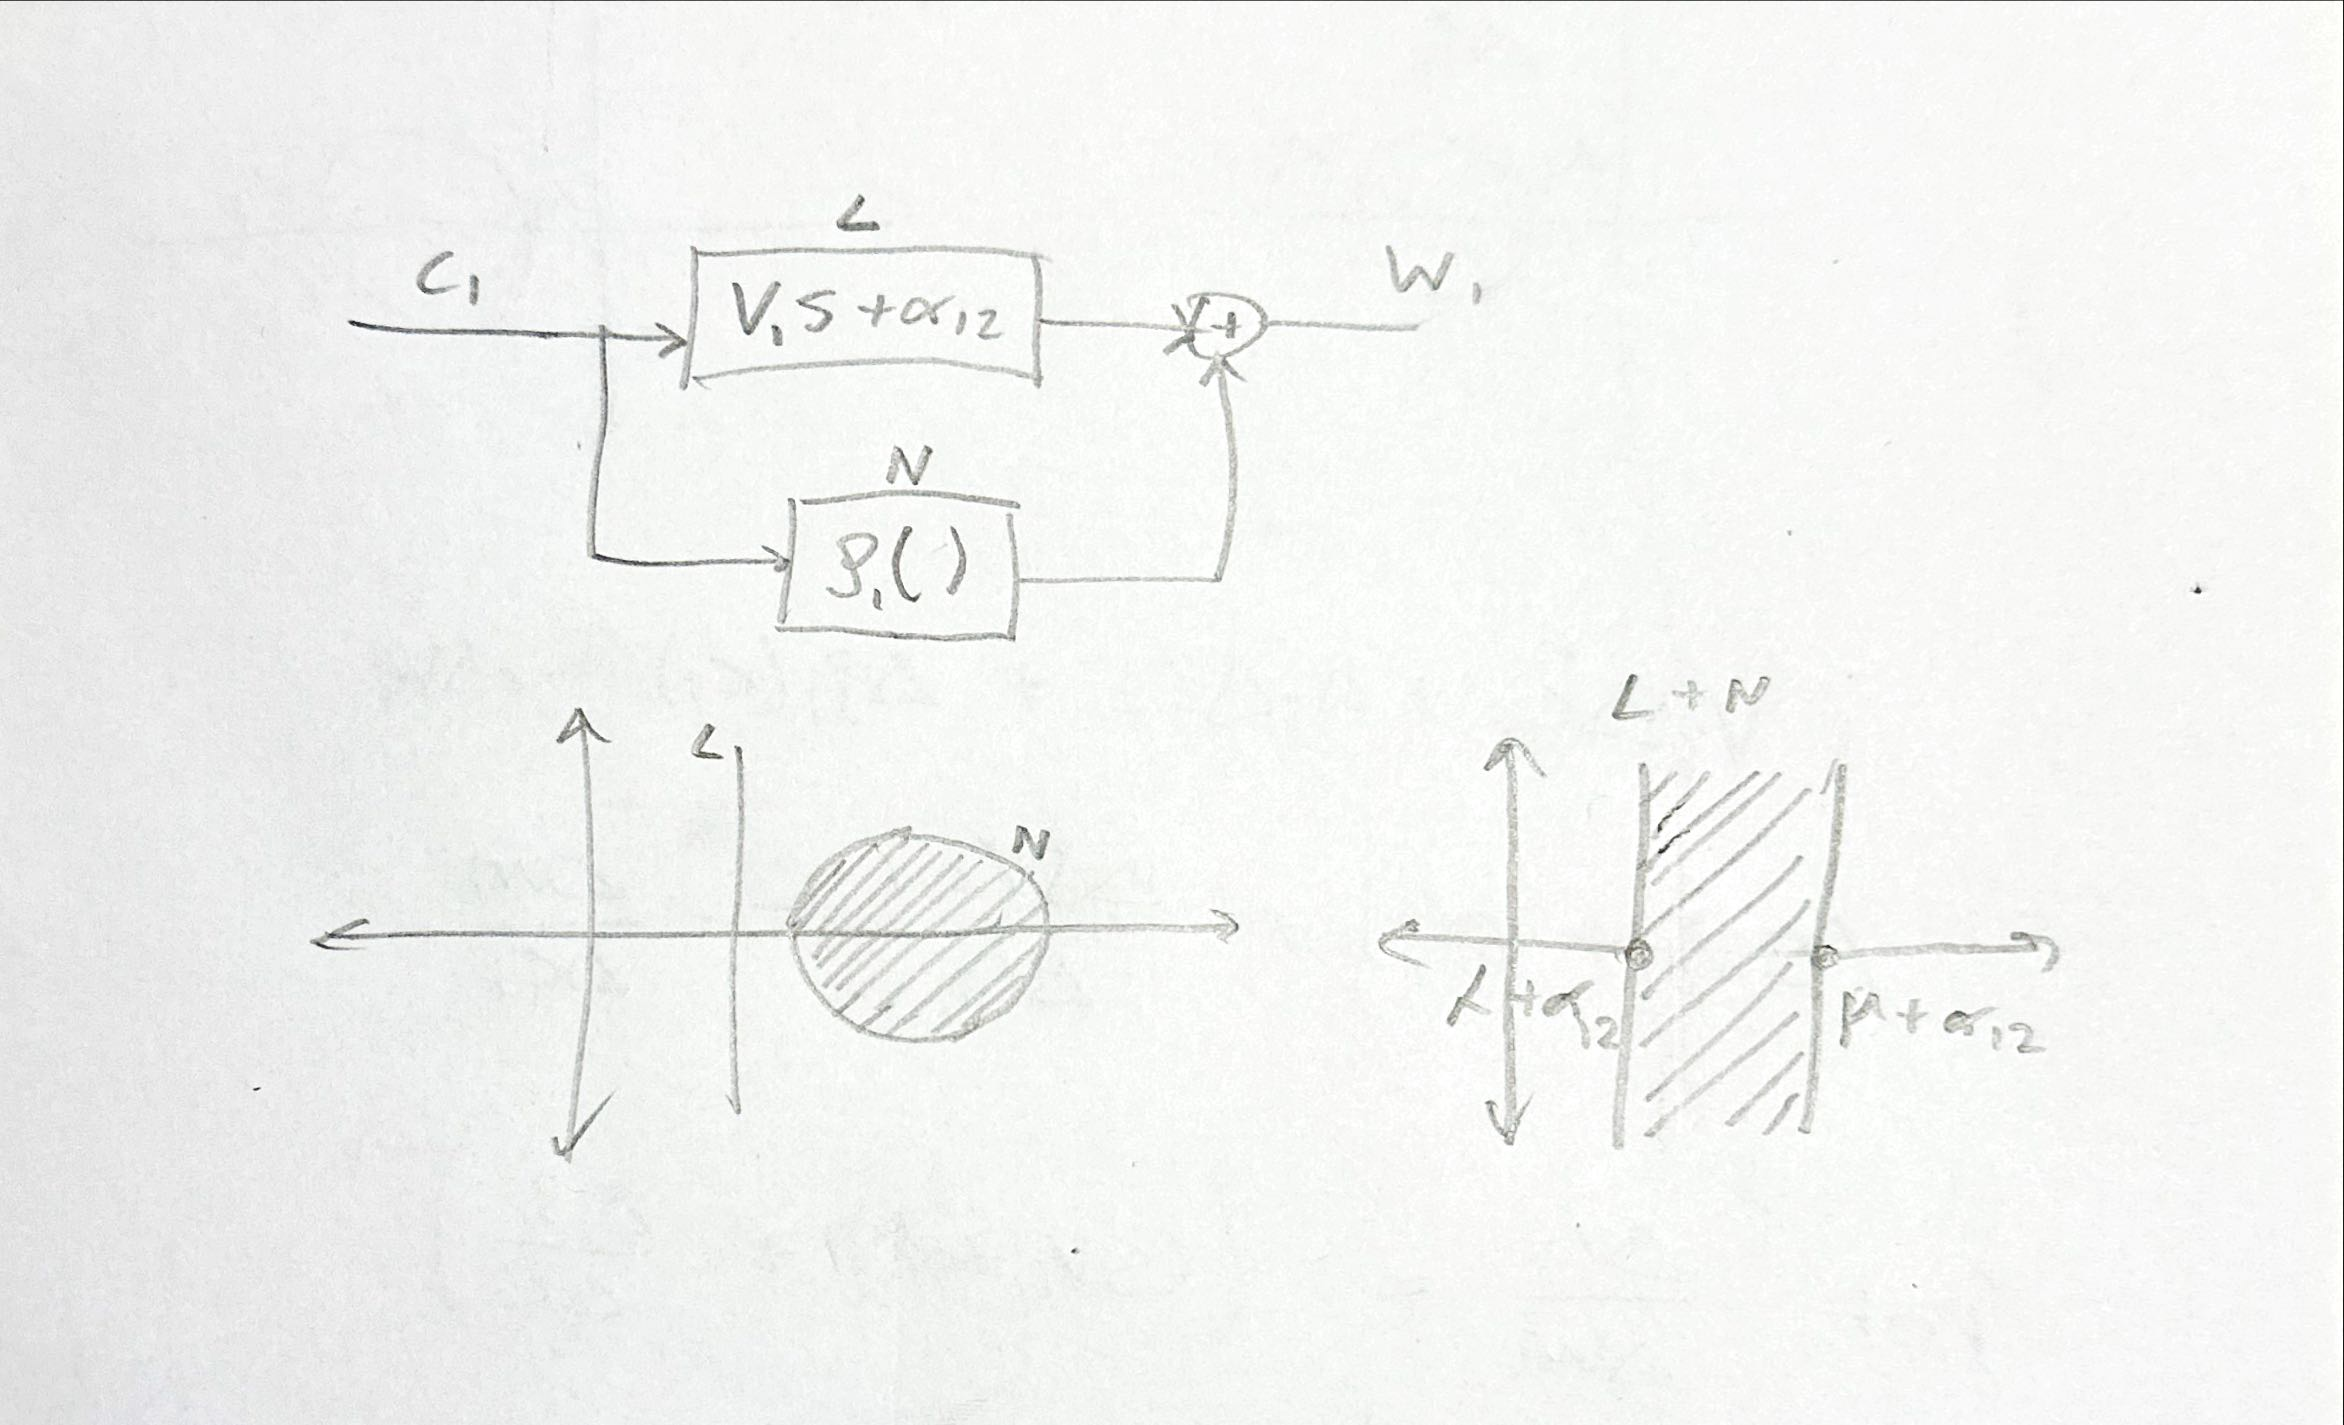
\includegraphics[width=0.4\textwidth]{figures/componentSRGs.jpg}
    \caption{Scaled Relative Graphs of sets L and N and their Minkowski sum}
\end{figure}
When inverted the resultant SRG is a larger circle between 0 and $1/(\lambda_1 + \alpha_{12})$ with a smaller circle removed from it between 0 and $1/(\mu_1 + \alpha_{12})$.
\begin{figure}[H]
    \centering
    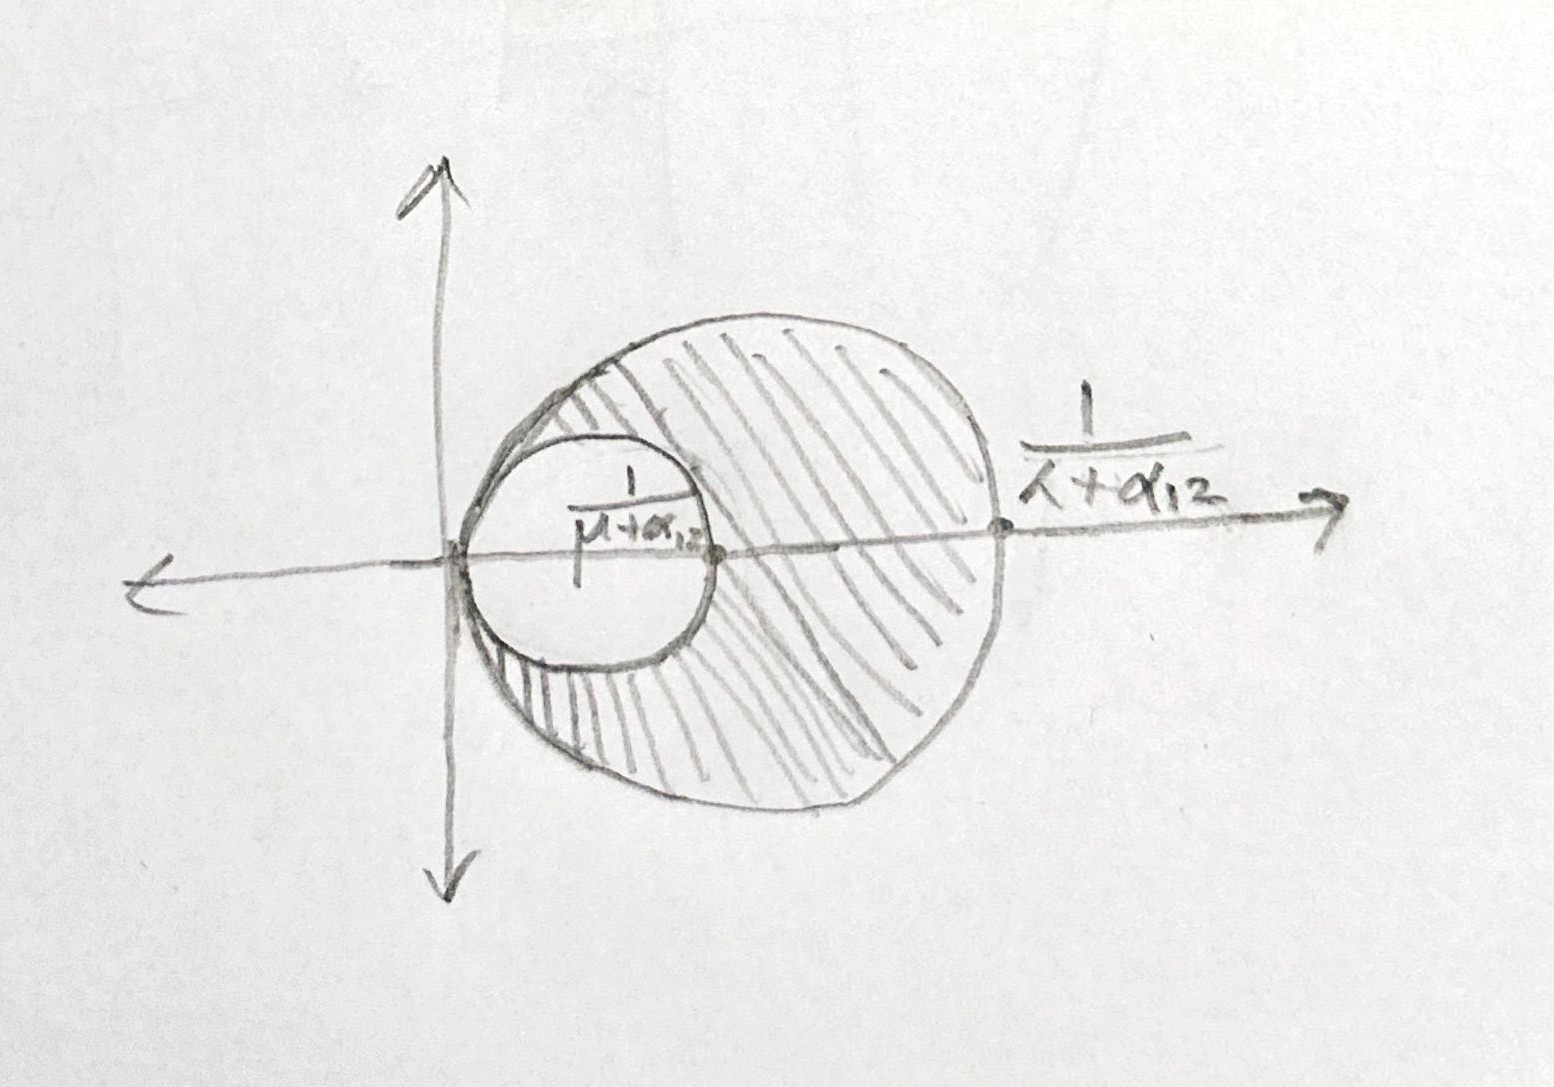
\includegraphics[width=0.4\textwidth]{figures/compartmentSRG.jpg}
    \caption{Scaled Relative Graph of component 1}
\end{figure}

\subsubsection{Positive feedback interconnection}

\begin{figure}[H]
    \centering
    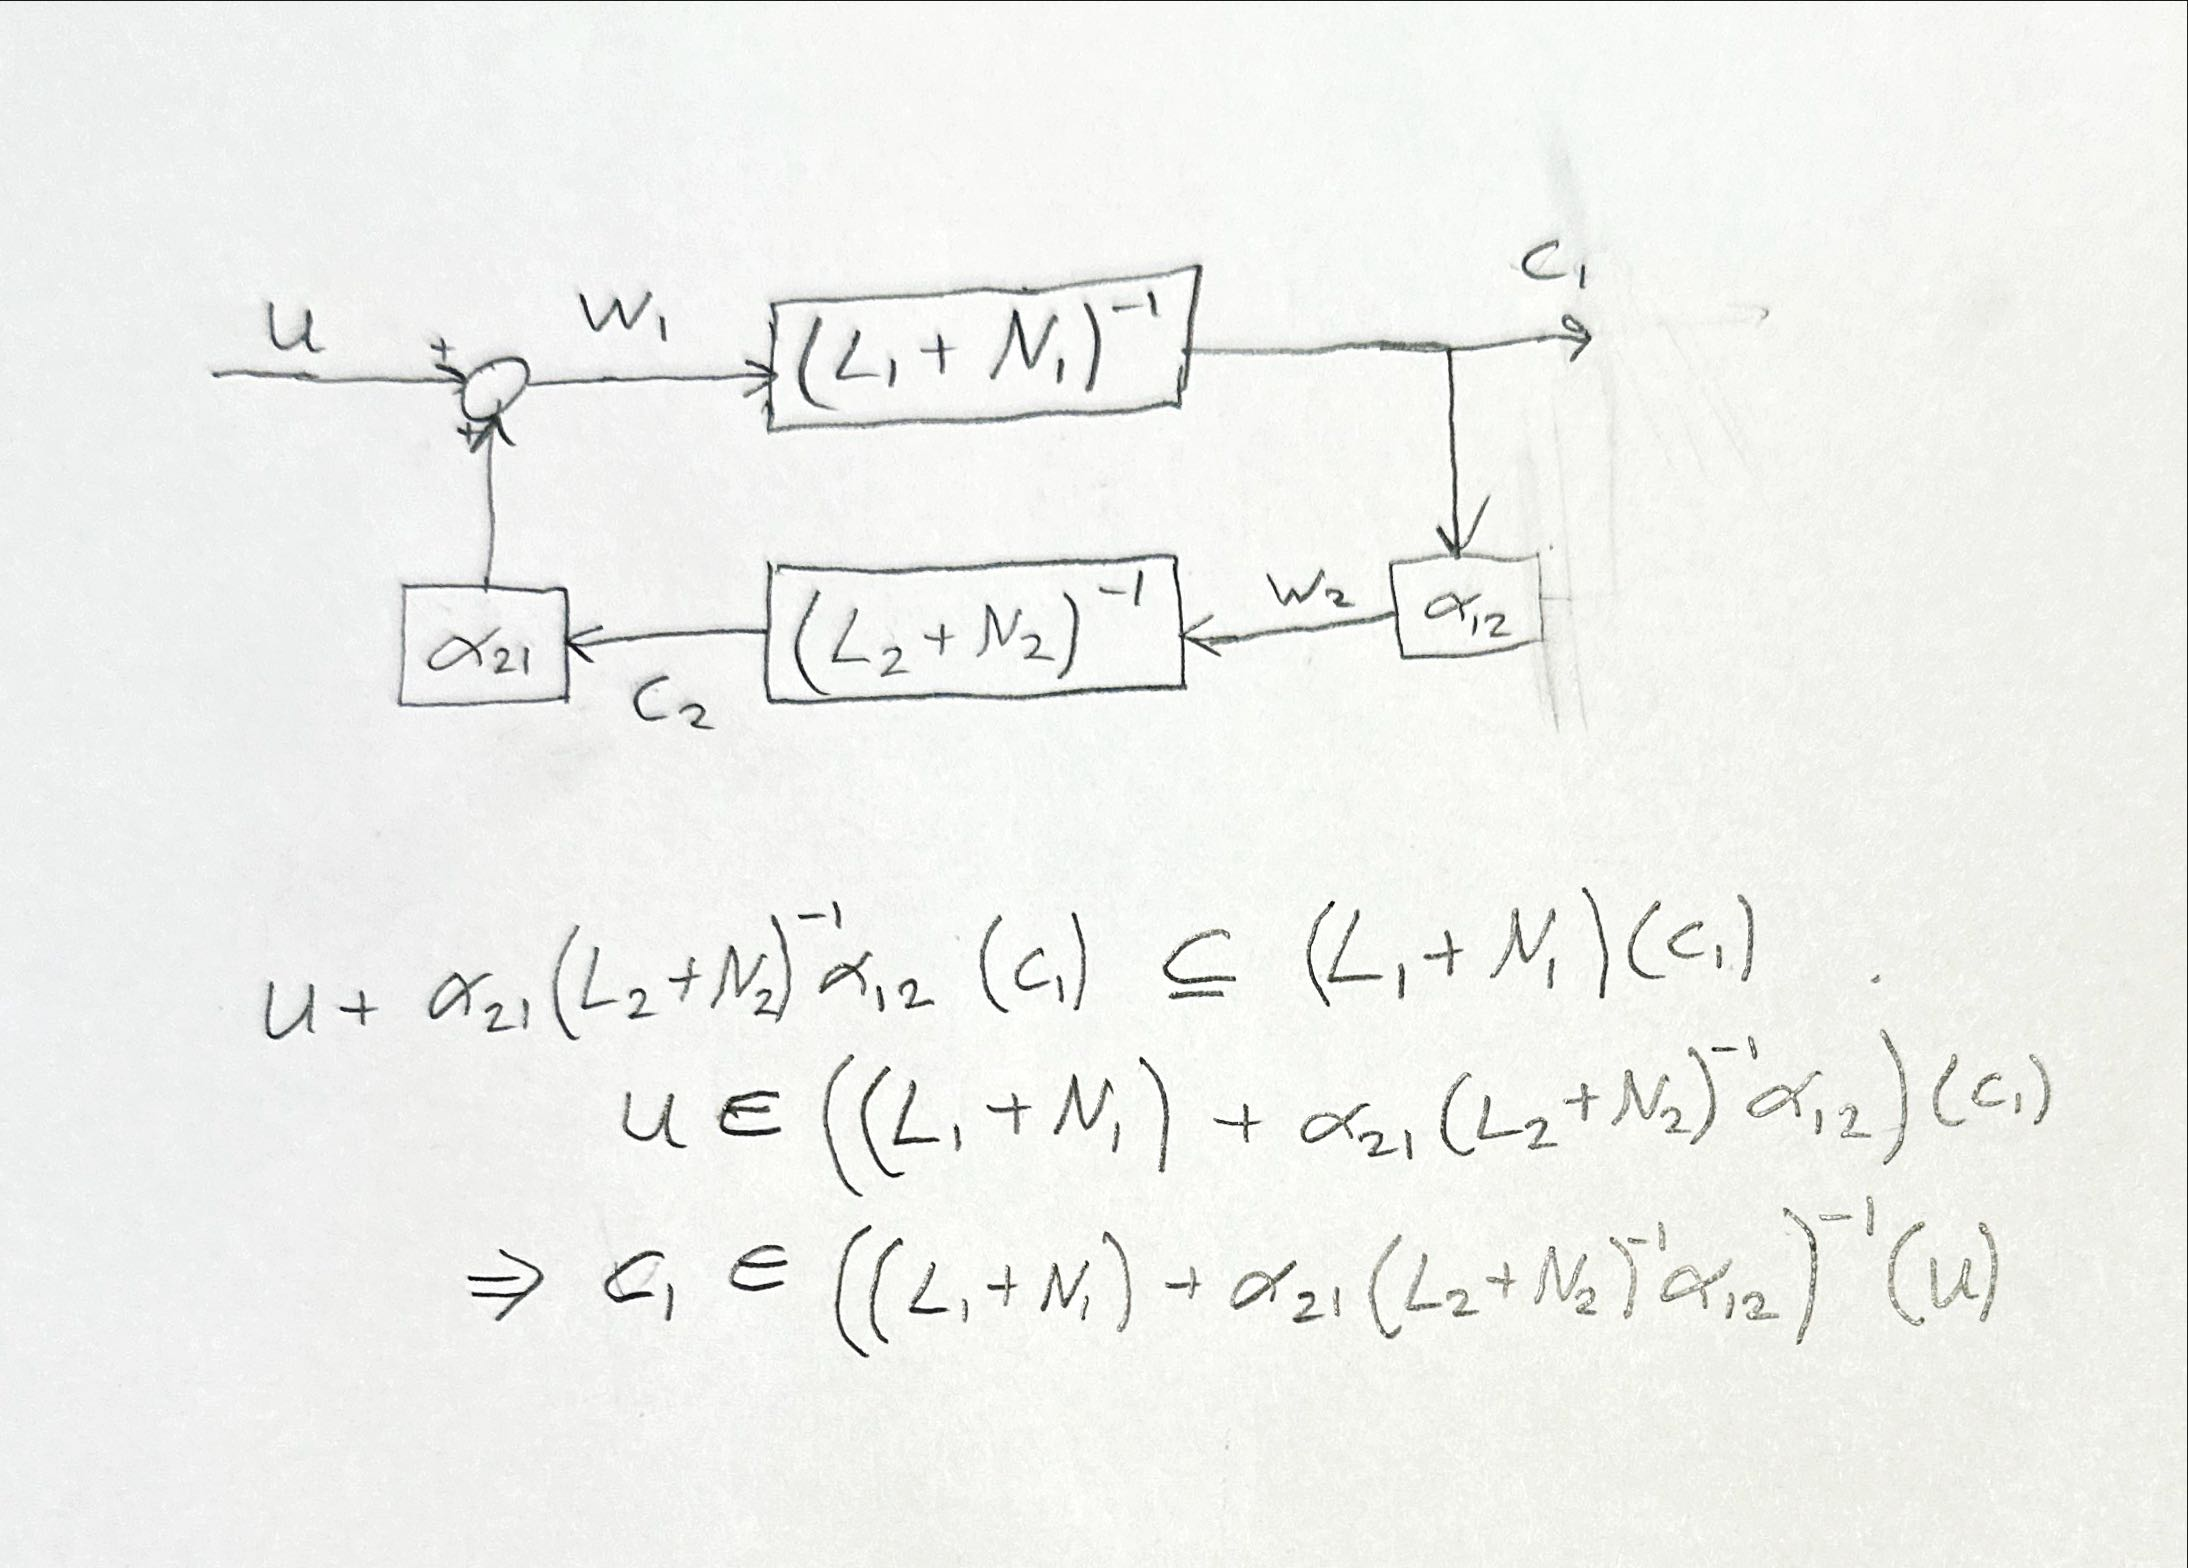
\includegraphics[width=0.4\textwidth]{figures/feedback_components.jpg}
    \caption{}
\end{figure}

\begin{figure}[H]
    \centering
    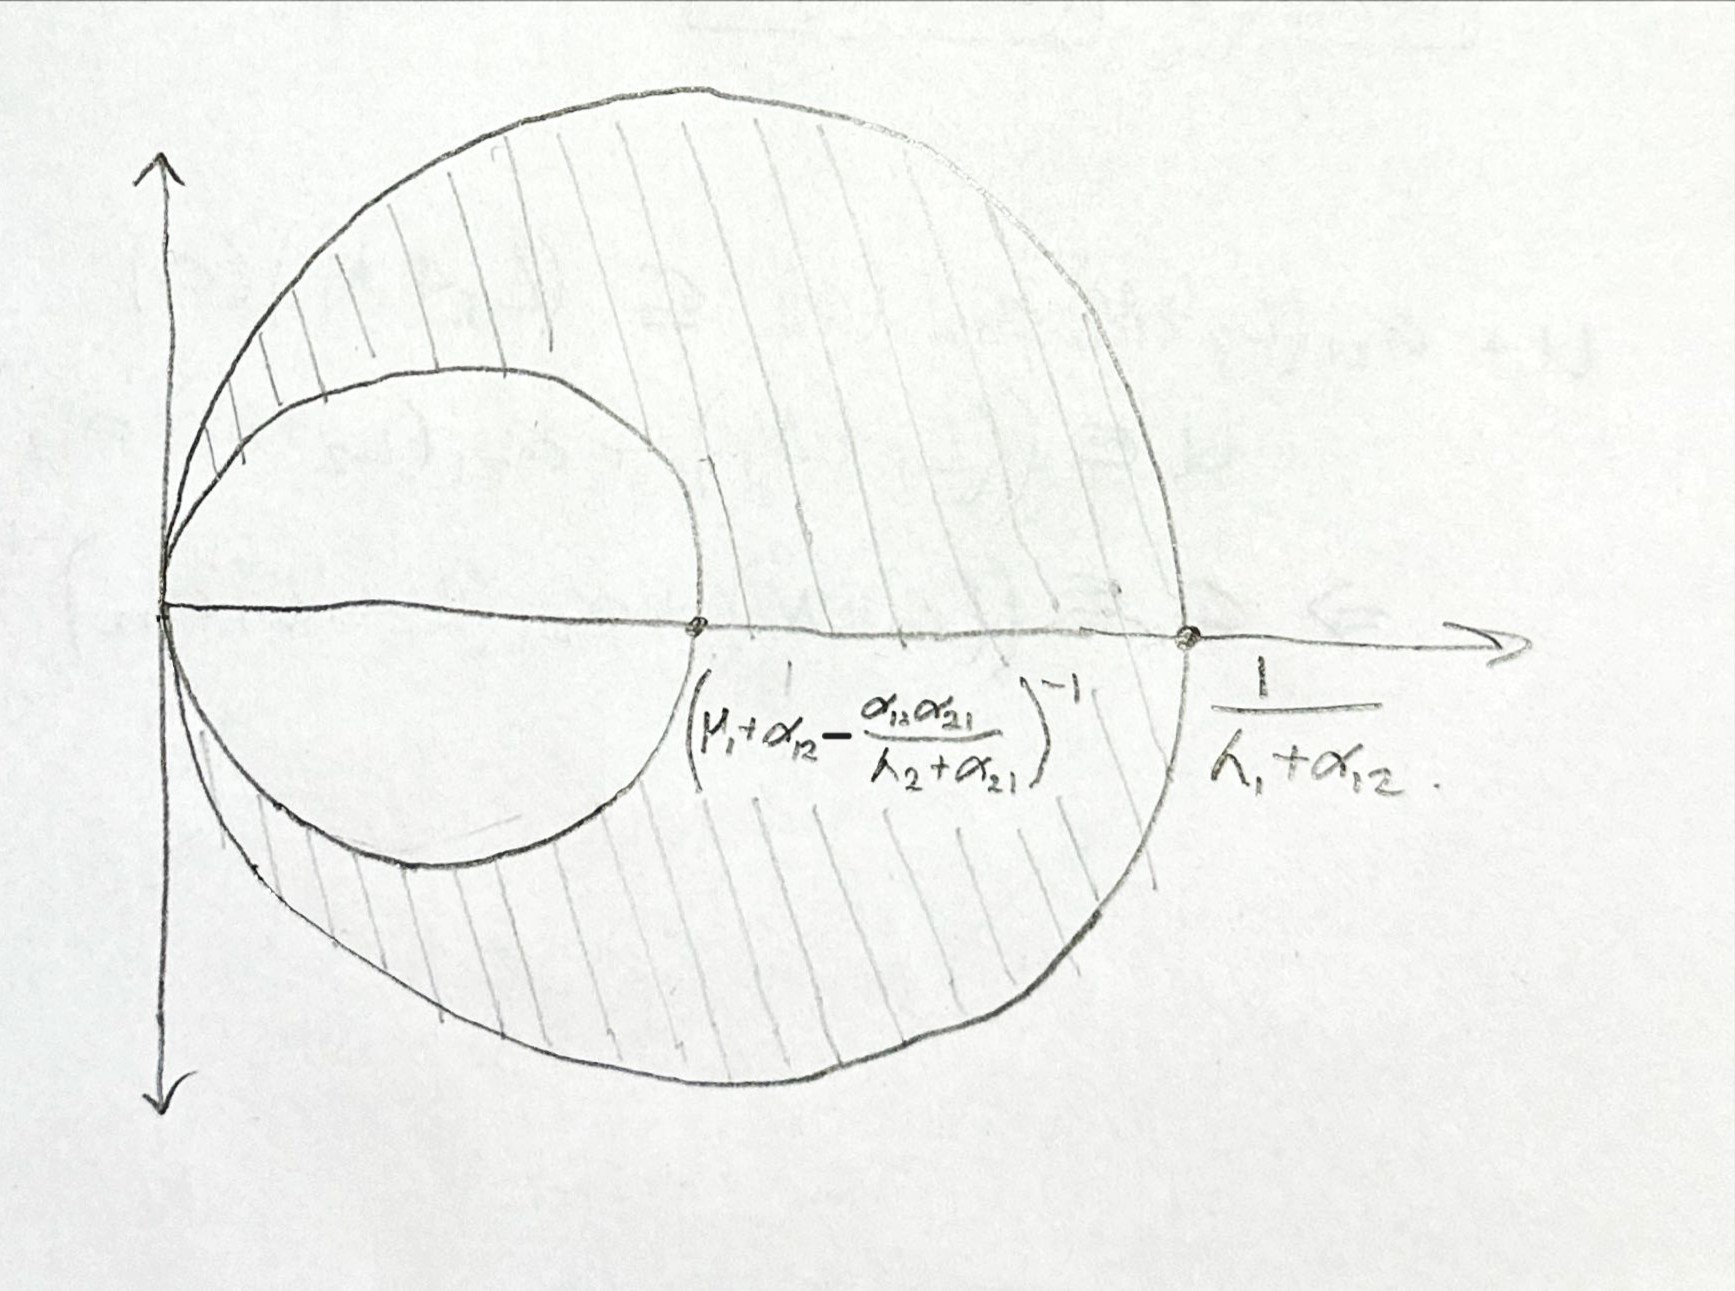
\includegraphics[width=0.4\textwidth]{figures/feedback_SRG.jpg}
    \caption{Scaled Relative Graph of positive feedback interconnection}
\end{figure}

\subsection{Automatic drug doses}

\subsubsection{Without sensor dynamics}

\begin{equation}
    u = k \text{ReLU}(r - y)
\end{equation}
\begin{equation}
    \text{ReLU}(x) = \begin{cases}
        x & \text{if } x > 0 \\
        0 & \text{otherwise}
    \end{cases}
\end{equation}
Which satisfies the incremental sector condition
\begin{equation}
    0 \leq k \frac{ReLU(x_1) - ReLU(x_2)}{x_1 - x_2} \leq k
\end{equation}

This means that the SRG of the controller can be represented by a disc between 0 and $k$.
The closed loop then consists of a cascade of the controller and plant.

\begin{figure}[H]
    \centering
    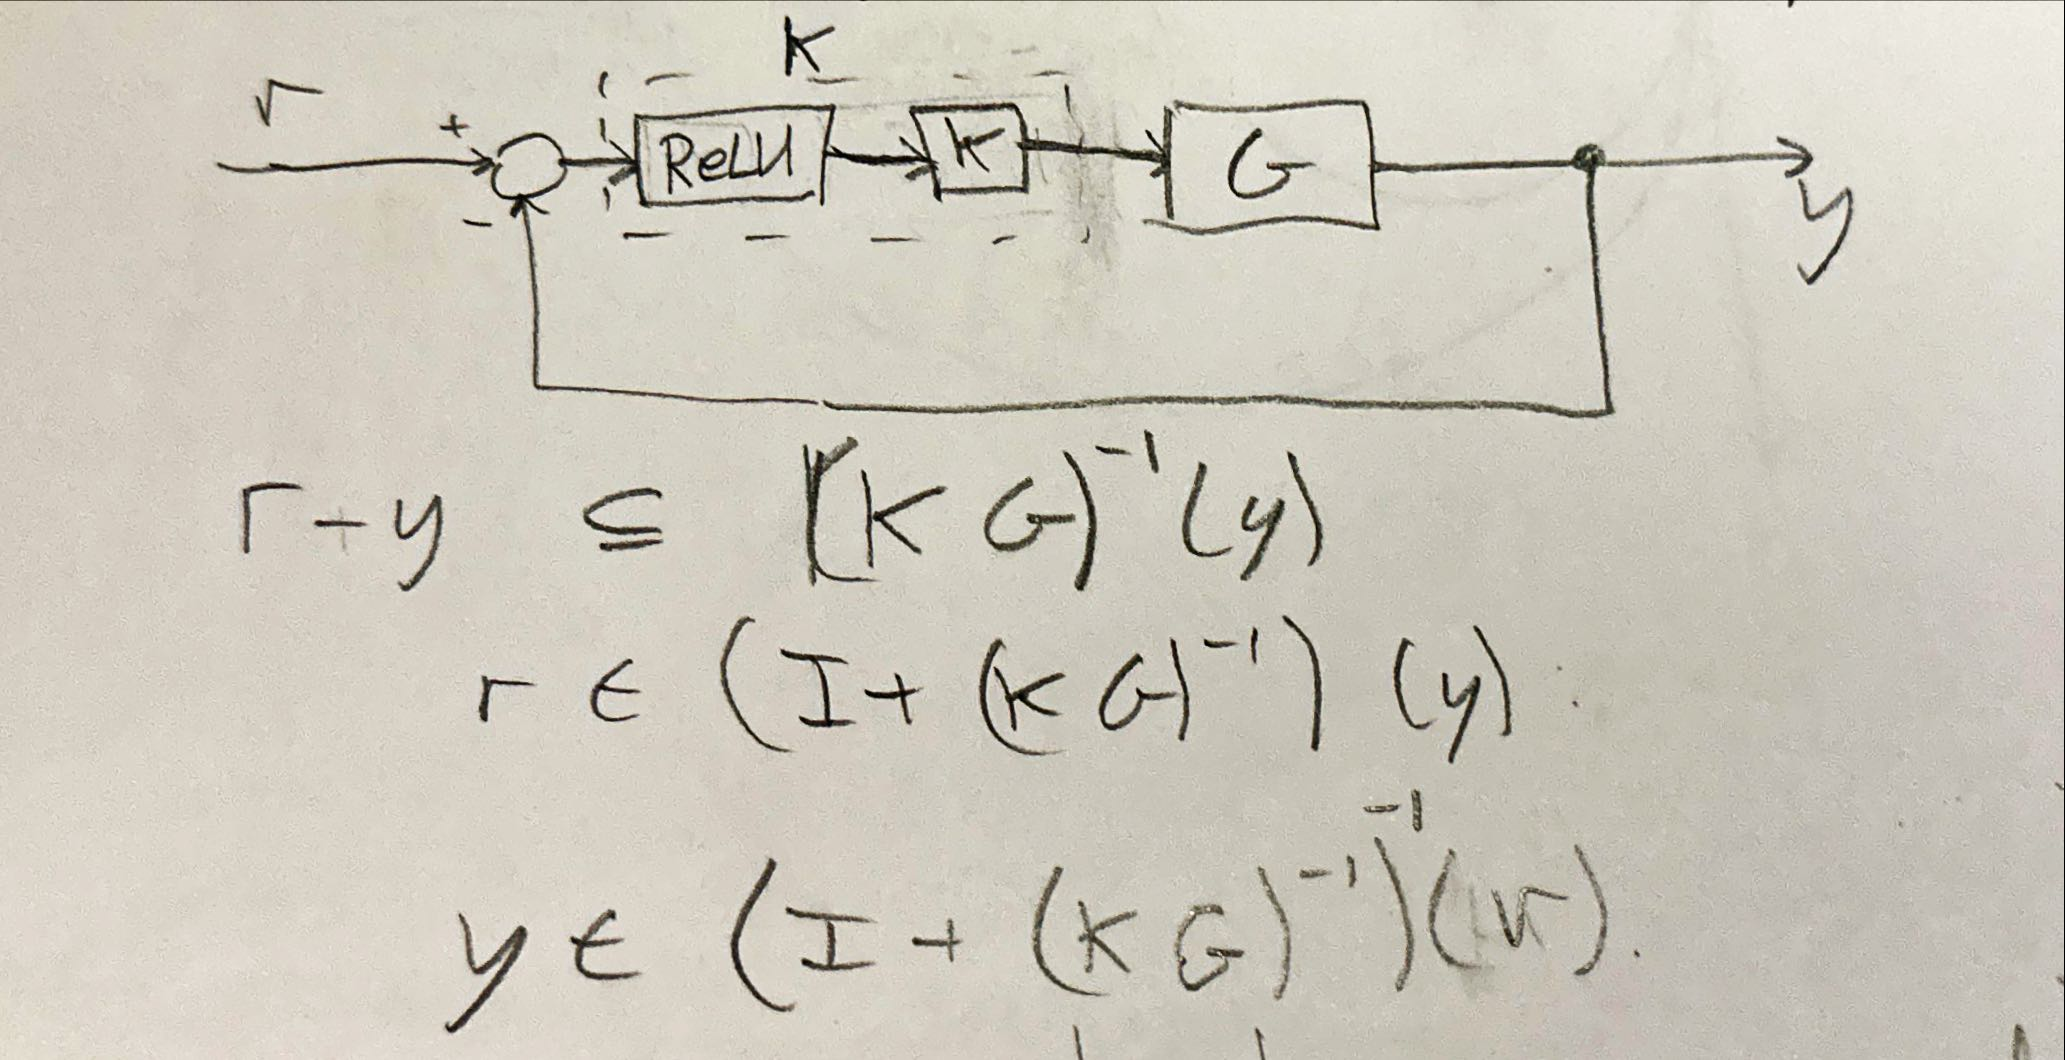
\includegraphics[width=0.5\textwidth]{figures/closed_loop.jpg}
    \caption{Closed loop block diagram}
\end{figure}
The SRG of the combined controller and plant forms a cardioid shape seen below.

\begin{figure}[H]
    \centering
    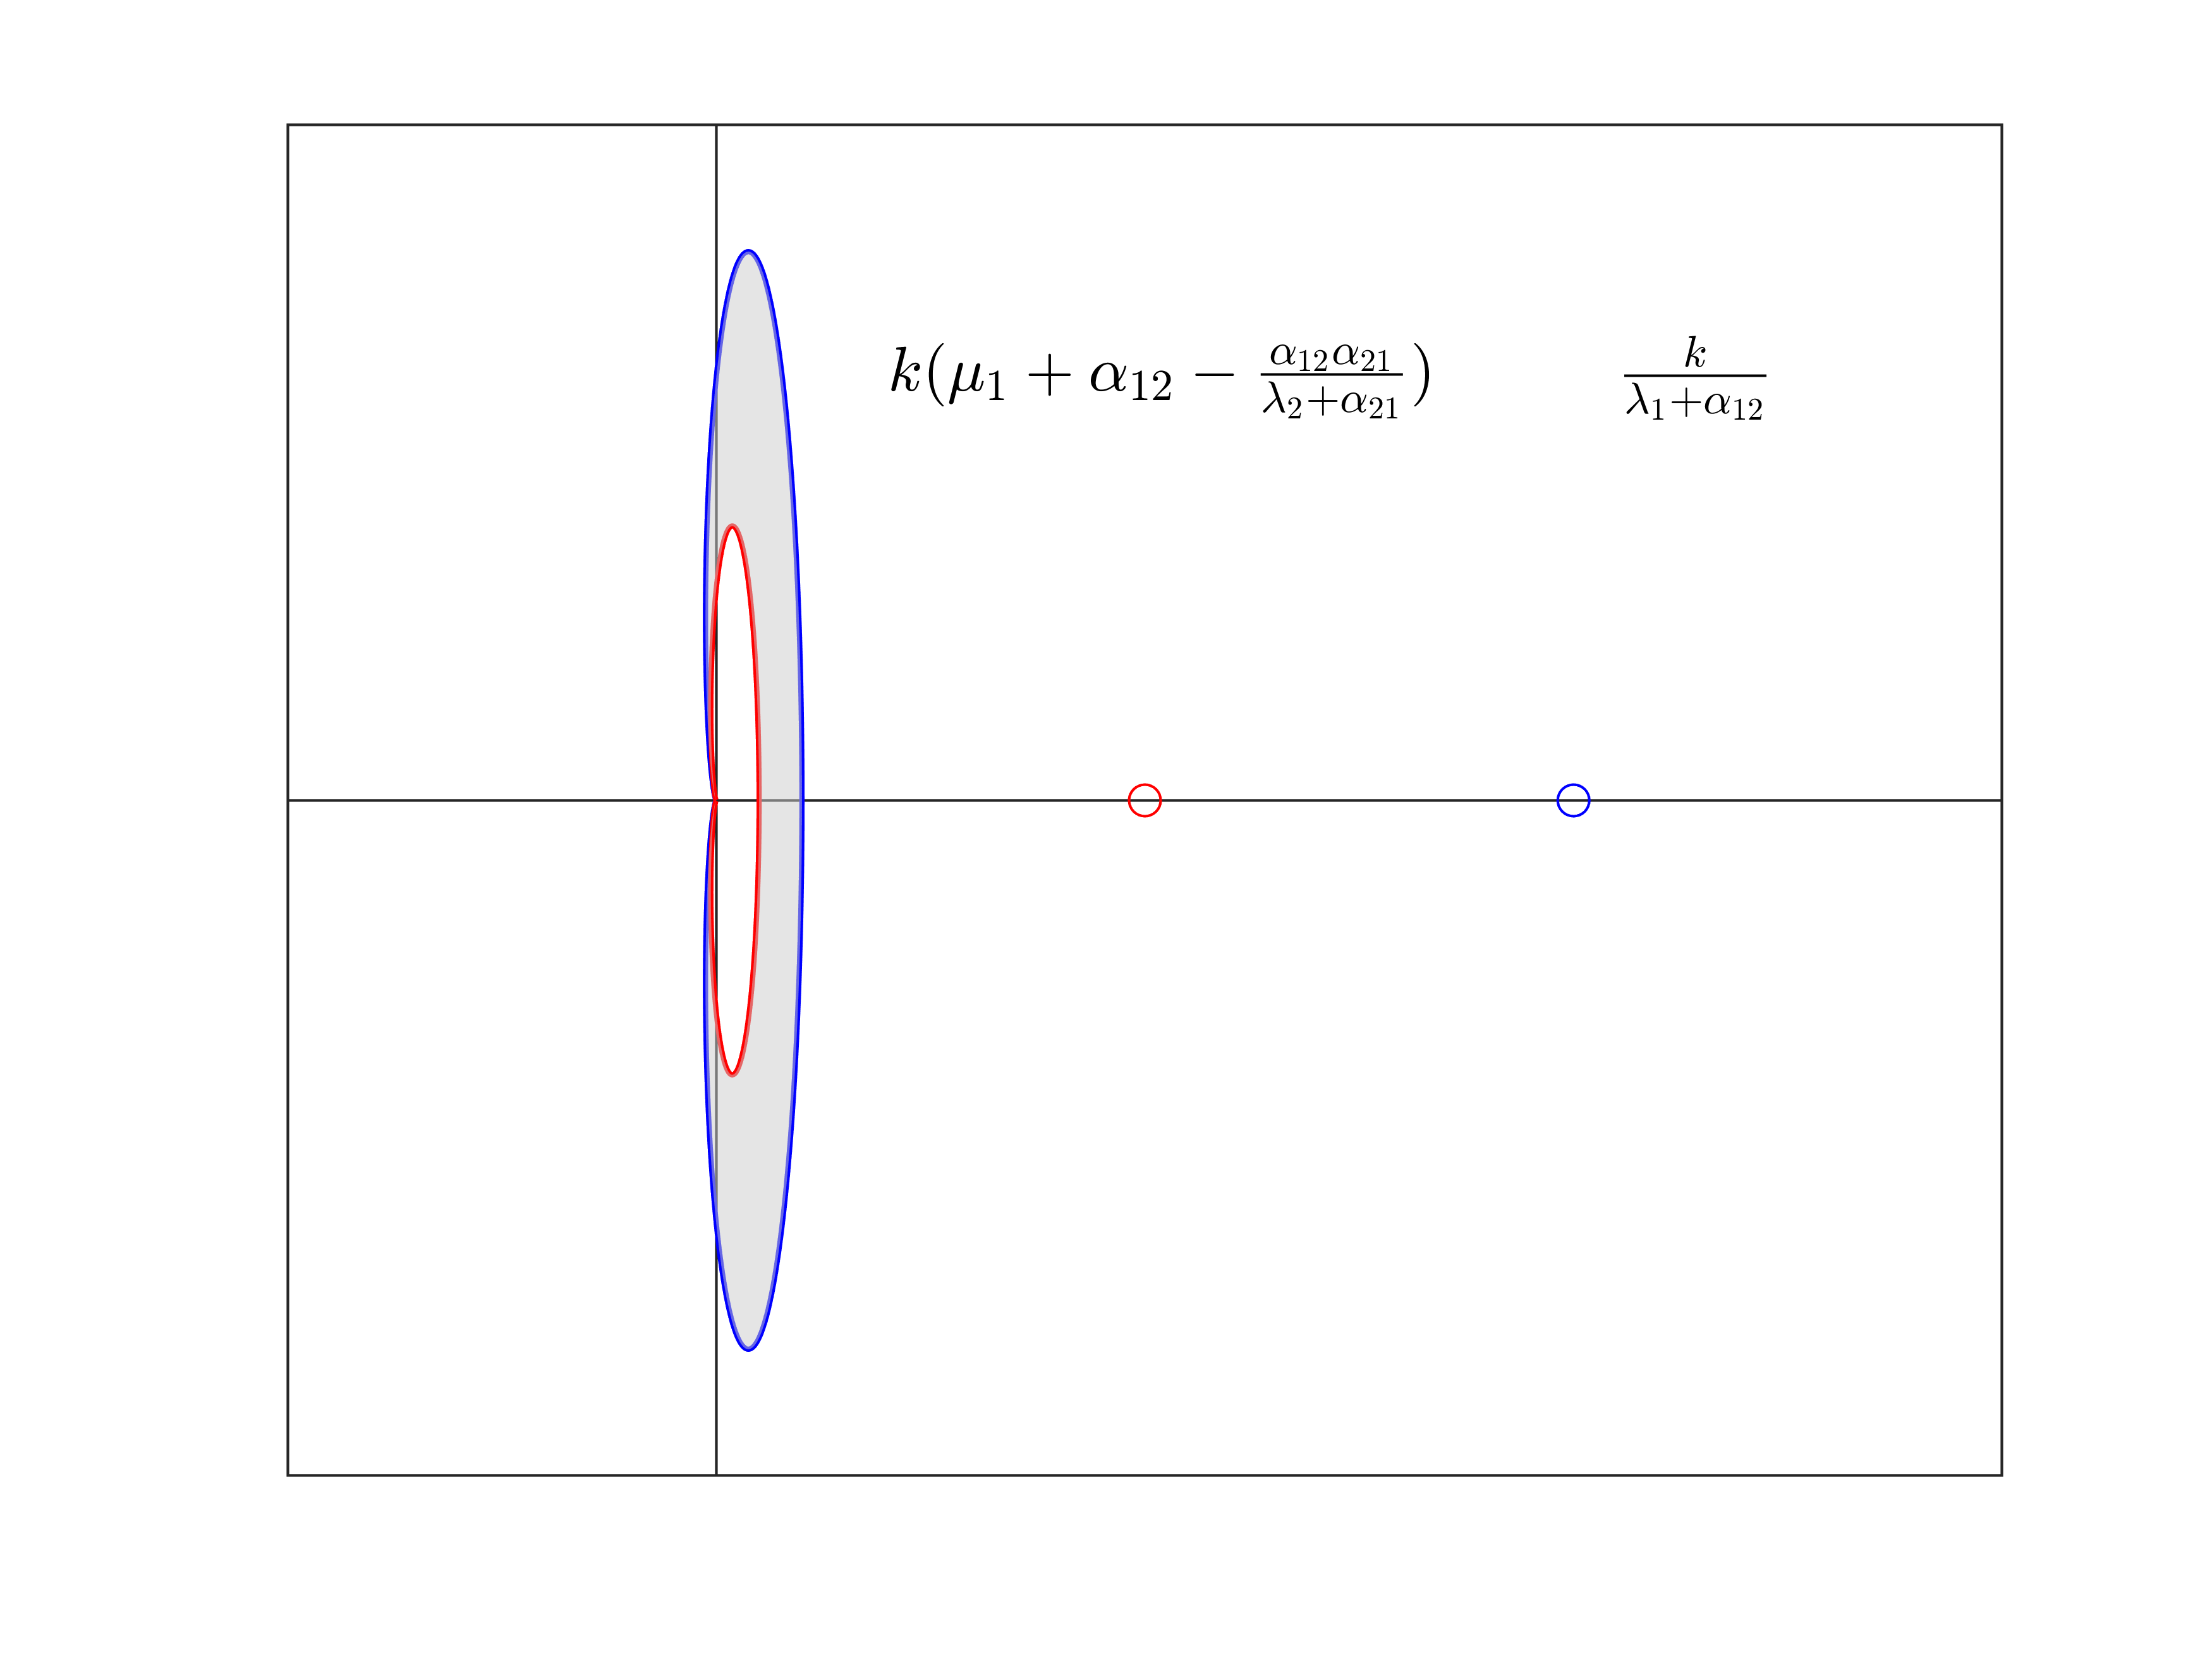
\includegraphics[width=0.5\textwidth]{figures/closed_loop_return_ratio.png}
    \caption{Scaled Relative Graph of closed loop return ratio}
    \label{fig:return_ratio_srg}
\end{figure}

For stability the Nonlinear Nyquist criterion is used.
%The closed loop system is stable if the number of encirclements of $-1$ by $kG(e^{j\theta})$ for $\theta \in [-\pi, \pi]$ equals the number of open loop unstable poles.
% should use the circle criterion.
%For determining the range of $k$ for stability, the Circle Criterion is used.
If $\text{SRG}(H_1^{-1})$ and -$\tau \text{SRG}(H_2)$ are separated by distance greater than $r_\text{min} > 0 \forall \tau \in [0,1]$.
Then the feedback interconnection of $H_1$ and $H_2$ has fading memory and incremental gain bound of $1/r_\text{min}$.
Considering $H_1$ as in figure \ref{fig:return_ratio_srg} and $H_2$ as 1 for $y=c_1$ means the distance from $H_1$ to the point $-\tau$.
This can be seen to satisfy the nonlinear Nyquist criterion for $k \geq 0$.

\subsubsection{With sensor dynamics}

The sensor has a time constant associated with it.

\begin{equation}
    \tau_s \dot{y} = -y + c_1
\end{equation}

This can be represented as an additional first order lag in the $H_2$ feedback interconnection.

\begin{figure}[H]
    \centering
    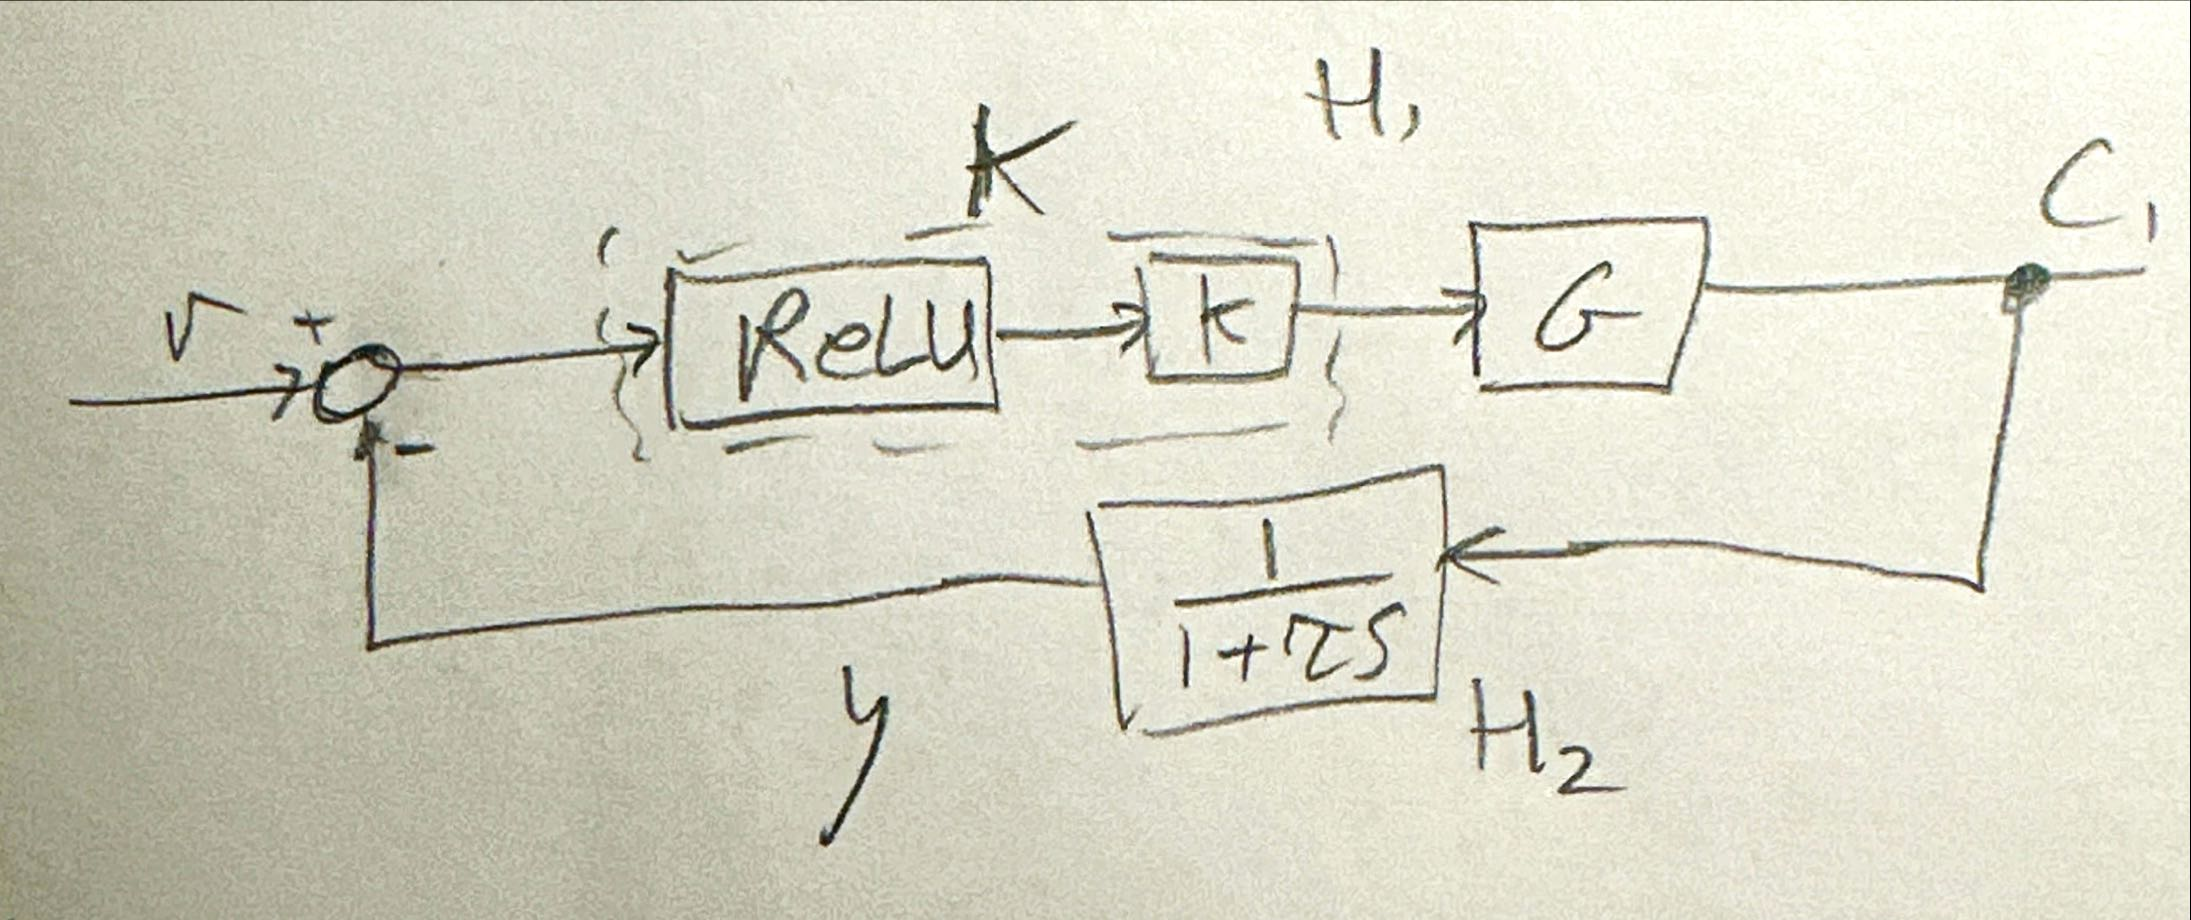
\includegraphics[width=0.5\textwidth]{figures/sensor_dynamics.jpg}
    \caption{Block diagram of system with sensor dynamics}
    \label{fig:sensor_dynamic_block}
\end{figure}

Both SRGs can be plot and the minimum distance $r_\text{min}$ between $H_1$ and $-\tau H_2 $ for $\tau \in [0,1]$ can be calculated.
% TODO: find the right answer for this
% somethings gone wrong earlier because for all tau>0 the SRGs overlap

\section{Appendix}


\begin{figure}[H]
    \centering
    \begin{lstlisting}
        cvx_begin sdp
            variable Y(n,n) symmetric
            variable Z(m,n)
            variable epsilon
            variable gama
            
            %minimise(gama)
            minimise(epsilon) % otherwise makes very high

            LMI1 = Y >= 0
            LMI2 = gama <= 0.1
            
            % gain LMI
            LMI3 = [ (Y*A' + A*Y + Z'*Bu' + Bu*Z),   (Y*Cz' + Z'*Dzu'),          Bw;
                    (Cz*Y + Dzu*Z),  -gama*eye(2),      Dzw';
                    Bw',            Dzw,                -gama*eye(2) ] <= 0;
            
            % passivity LMI
            LMI4 = epsilon >= 0
            LMI5 = [ Y*A' + A*Y + Bu*Z + Z'*Bu', Bw - Y*Cy' - Z'*Dyu';
                    Bw' - Cy*Y-Dyu*Z,   -2*epsilon*eye(2) - (Dyw + Dyw')] <= 0
                
        cvx_end
    \end{lstlisting}
    \caption{CVX code for bounded gain and passivity controller}
    \label{fig:bounded_passive_lmi}
\end{figure}

\begin{thebibliography}{9}

    %Endres, SC, Sandrock, C, Focke, WW (2018) “A simplicial homology algorithm for lipschitz optimisation”, Journal of Global Optimization.
    
      \bibitem{handout}
      F. Forni, R, Sepulchre
      \emph{4F2, Robust and Nonlinear Control: Coursework 1}
      University of Cambridge,
      2025.

      \bibitem{lecture}
      F. Forni
      \emph{4F2, Robust and Nonlinear Control: Handout 6}
      University of Cambridge,
      2025.
    
      \bibitem{matlab_robustmu}
      MATLAB
      \emph{Robust Performance Measure for Mu Synthesis}
      \texttt{https://uk.mathworks.com/help/robust/ug/measures-of-robust-performance.html}

    
\end{thebibliography}

\end{document}